% Appendices are set up same as chapter sections
\chapter{Appendix - Additional Design Development}

\section{Dark horse}
\subsection{Dark Horse Version 1}
\subsubsection{Benchmarking}
Our vision for what we wanted to accomplish with our Dark Horse prototype led us to examine different possible cabin configurations and other ways to use the space inside the cabin without current seat constraints. Our team brainstormed a number of different activities that could take place during flight, shown in Figure \ref{fig:possible_themes.jpg}, which would enable passengers to have a much more personalized and enjoyable experience. 

\begin{figure}[h]
  \centering
     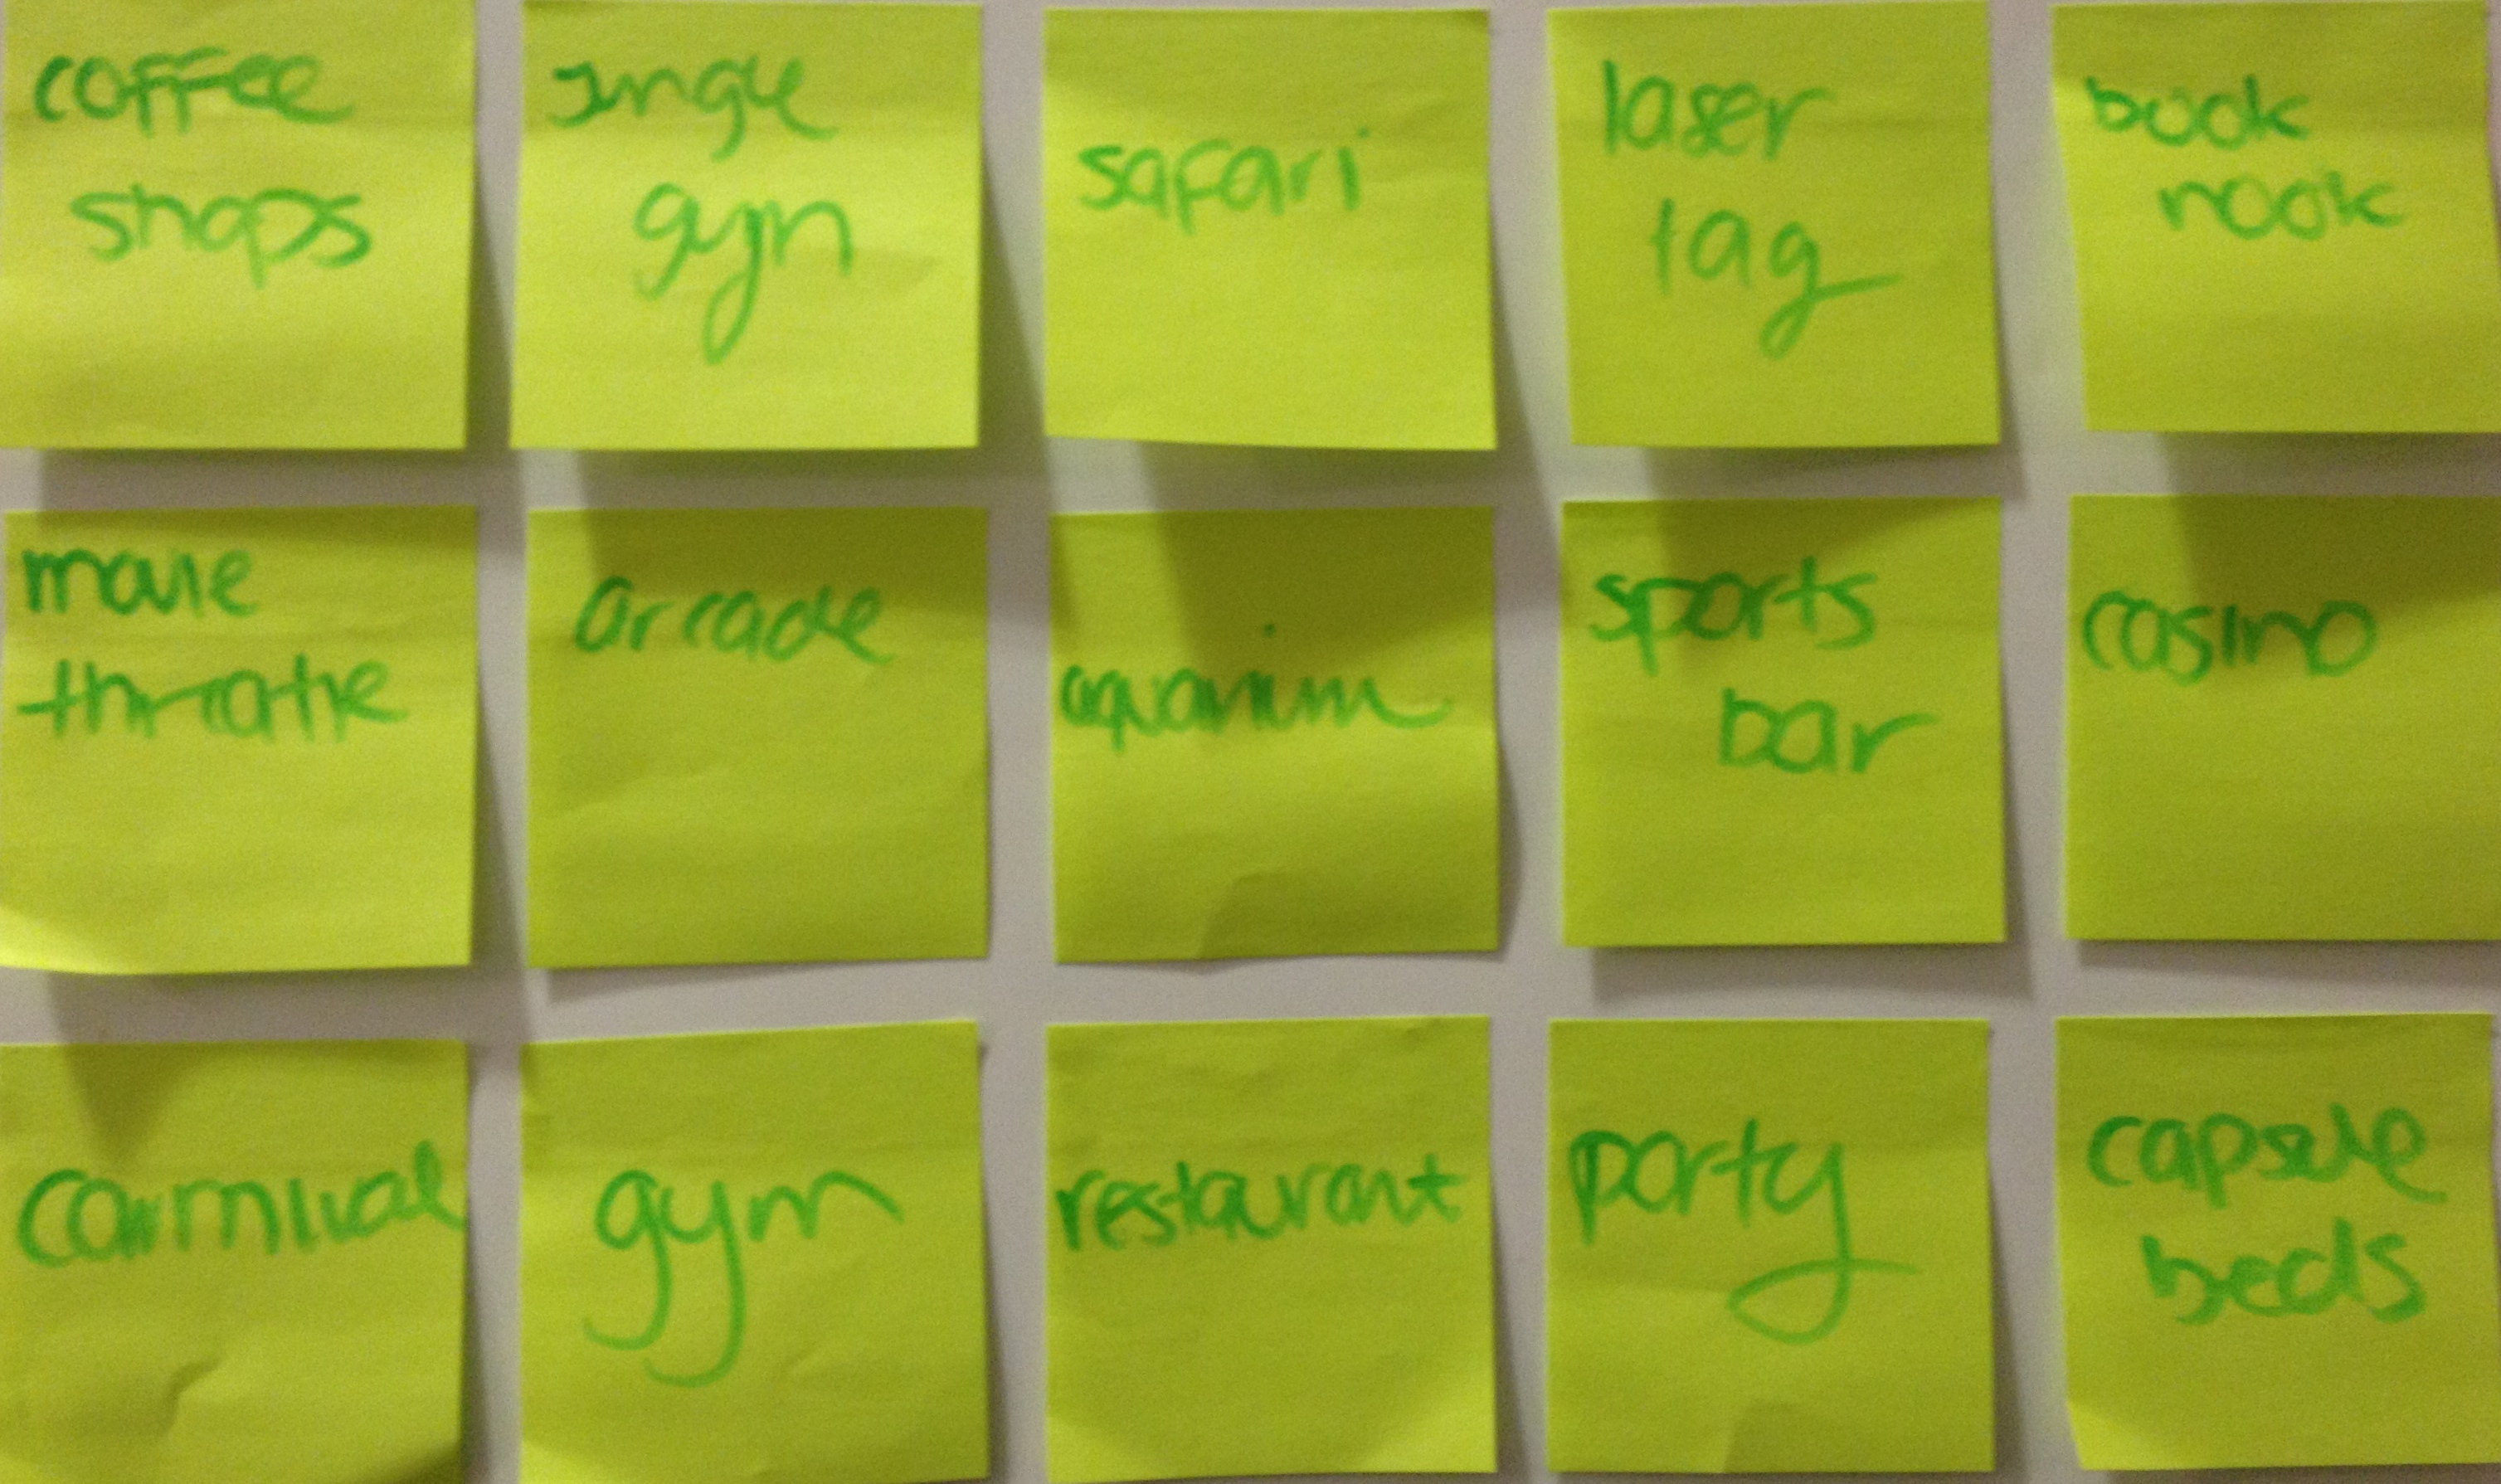
\includegraphics[width=7cm]{images/possible_themes.jpg}
   \caption{Possible ideas for a new cabin configuration}
  \label{fig:possible_themes.jpg}
\end{figure}

Our goal for the first Dark Horse Prototype was to find ways to make flying an enjoyable activity, not just another form of transportation. While many passengers find that getting to and around the airport, going through security, and waiting for a flight to board can be a waste of time and a draining activity, people are willing to pay to stand in line at theme parks for hours on end just to get on a fun ride for a few minutes or camp out outside of stores just to get the new iPhone. We believe that if we could make the flying experience a better one, passengers would be less bothered by the less-than-pleasant activities leading up to it. 

We realized that a redesigned cabin would need to be more accessible but could also have different sections explicitly to harness our users’ varied needs and reasons for flying. Flying tends to be a time for rest for many and because of this we researched what others had done to convert the cabin from a “sitting room only” configuration to a more sleep-friendly space. One of the proxies we looked at were the pod hotels in Japan, shown in Figure \ref{fig:hotel_pod.jpg}, where people sleep in fairly compact space-efficient pods. Similar pods could be designed for use in an airplane cabin, reappropriating room typically used for seating to sleeping spaces.

\begin{figure}[h]
  \centering
     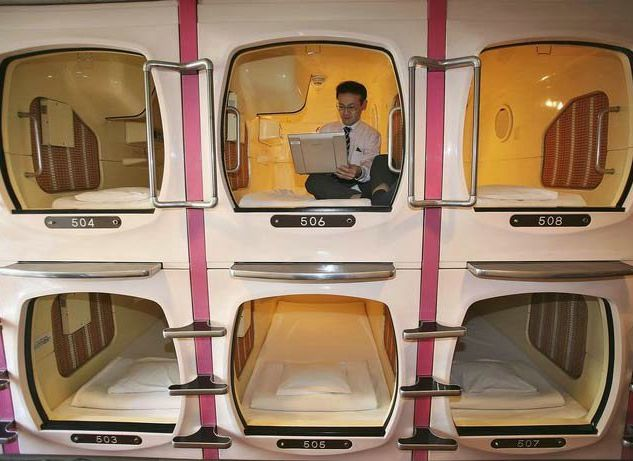
\includegraphics[width=7cm]{images/hotel_pod.jpg}
   \caption{Current pod hotel layout in Japan. Source: http://montaraventures.com/blog/2008/06/08/pod-hotel/}
  \label{fig:hotel_pod.jpg}
\end{figure}

There are a number of possible airplane configurations for converting the whole airplane into beds. This could be done by utilizing the vertical space available in the cabin, as shown in Figures \ref{fig:blue_vertical_configuration.png} and \ref{fig:blue_vertical_configuration.png}. 

\begin{figure}[h]
  \centering
     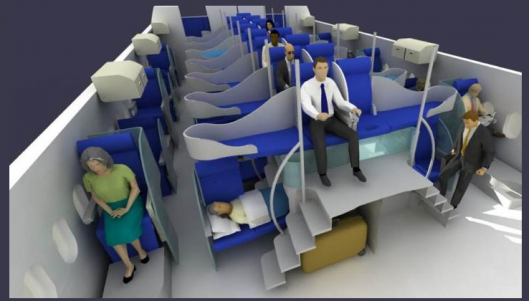
\includegraphics[width=7cm]{images/blue_vertical_configuration.png}
   \caption{Example of cabin layout that integrates both chairs and beds and does not decrease the total number of seats. Source: http://www.gizmag.com/future-of-air-travel-comfortable-seating/17751/}
  \label{fig:blue_vertical_configuration.png}
\end{figure} 

\begin{figure}[h]
  \centering
     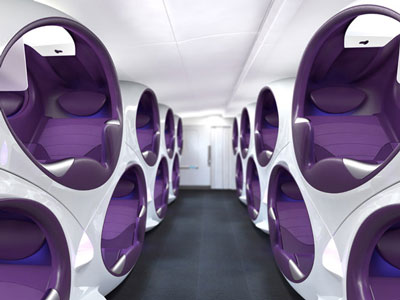
\includegraphics[width=7cm]{images/purple_vertical_configuration.jpg}
   \caption{Example of cabin layout with built in beds. Source: http://www.aviationinsurors.com/chair.html}
  \label{fig:purple_vertical_configuration.png}
\end{figure} 

These configurations make the flying experience much more comfortable while at the same time enabling selective seats to be much more accessible than others. These configurations would allow our users to easily get in and out of their seats without facing the problems they face today.

Our team also explored the possibility of sleeping while standing as opposed to laying down and found that there are several design firms that have been exploring vertical seating arrangements like the one shown in Figure \ref{fig:vertical_seating.jpg}. These designs have received a lot of backlash due to their perceived disregard for passenger comfort despite the fact that they may actually be better for our health. 

\begin{figure}[h]
  \centering
     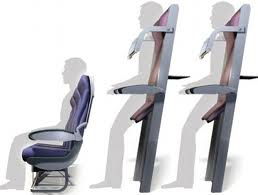
\includegraphics[width=7cm]{images/vertical_seating.jpg}
   \caption{Vertical seating being designed for airplane chairs. Source: http://www.dailymail.co.uk/news/article-1215081/Packed-like-sardines-New-aircraft-design-plans-seat-passengers-face-face.html}
  \label{fig:vertical_seating.jpg}
\end{figure} 

We know that many of our users travel for work purposes so we also considered what the best places to comfortably do work are and found that many preferred coffee shops to their offices. Our team also thought about having a gym integrated during the flight, transforming that seemingly lost flight time into a productive workout. Finally, we looked at different products available for creating a more accessible experience, including handles, conveyor belts and revolving doors. From all of this research, we created our first Dark Horse prototypes.

\subsubsection{Description of the prototype}
In order to make our users think about the present and not only their future destination we wanted to build a flexible and dynamic cabin layout enabling a more customized flight experience for everyone, especially handicapped passengers. \\

We made the assumption that when passengers buy their tickets, they will have to go through a questionnaire asking them for their preferred activity during the flight. According to their answers they will be placed in the appropriate section of the plane and have the opportunity to do what they really want to do during the flight. If the passengers have special needs due to physical handicaps, we wanted each of our different sections to address these issues and improve the experience not only for everyone, but in particular for those with reduced mobility. \\

Our team decided to focus on the design of 5 main sections and built a dynamic scale model for each one:

\subsubsection{Sleeping Area}
We wanted our user to be able to rest and relax so we thought of different types of beds or resting pods as mentioned in the benchmarking section. However, when we tried to prototype them and build our scale model we found at that it was quite hard to keep the number of seats the same. In order to not violate this constraint, our team decided to explore solutions that require a very limited space. As such, we designed our sleeping section with foldable seats which can be unfolded to become a bed as shown on the next picture.

\begin{figure}[h]
  \centering
     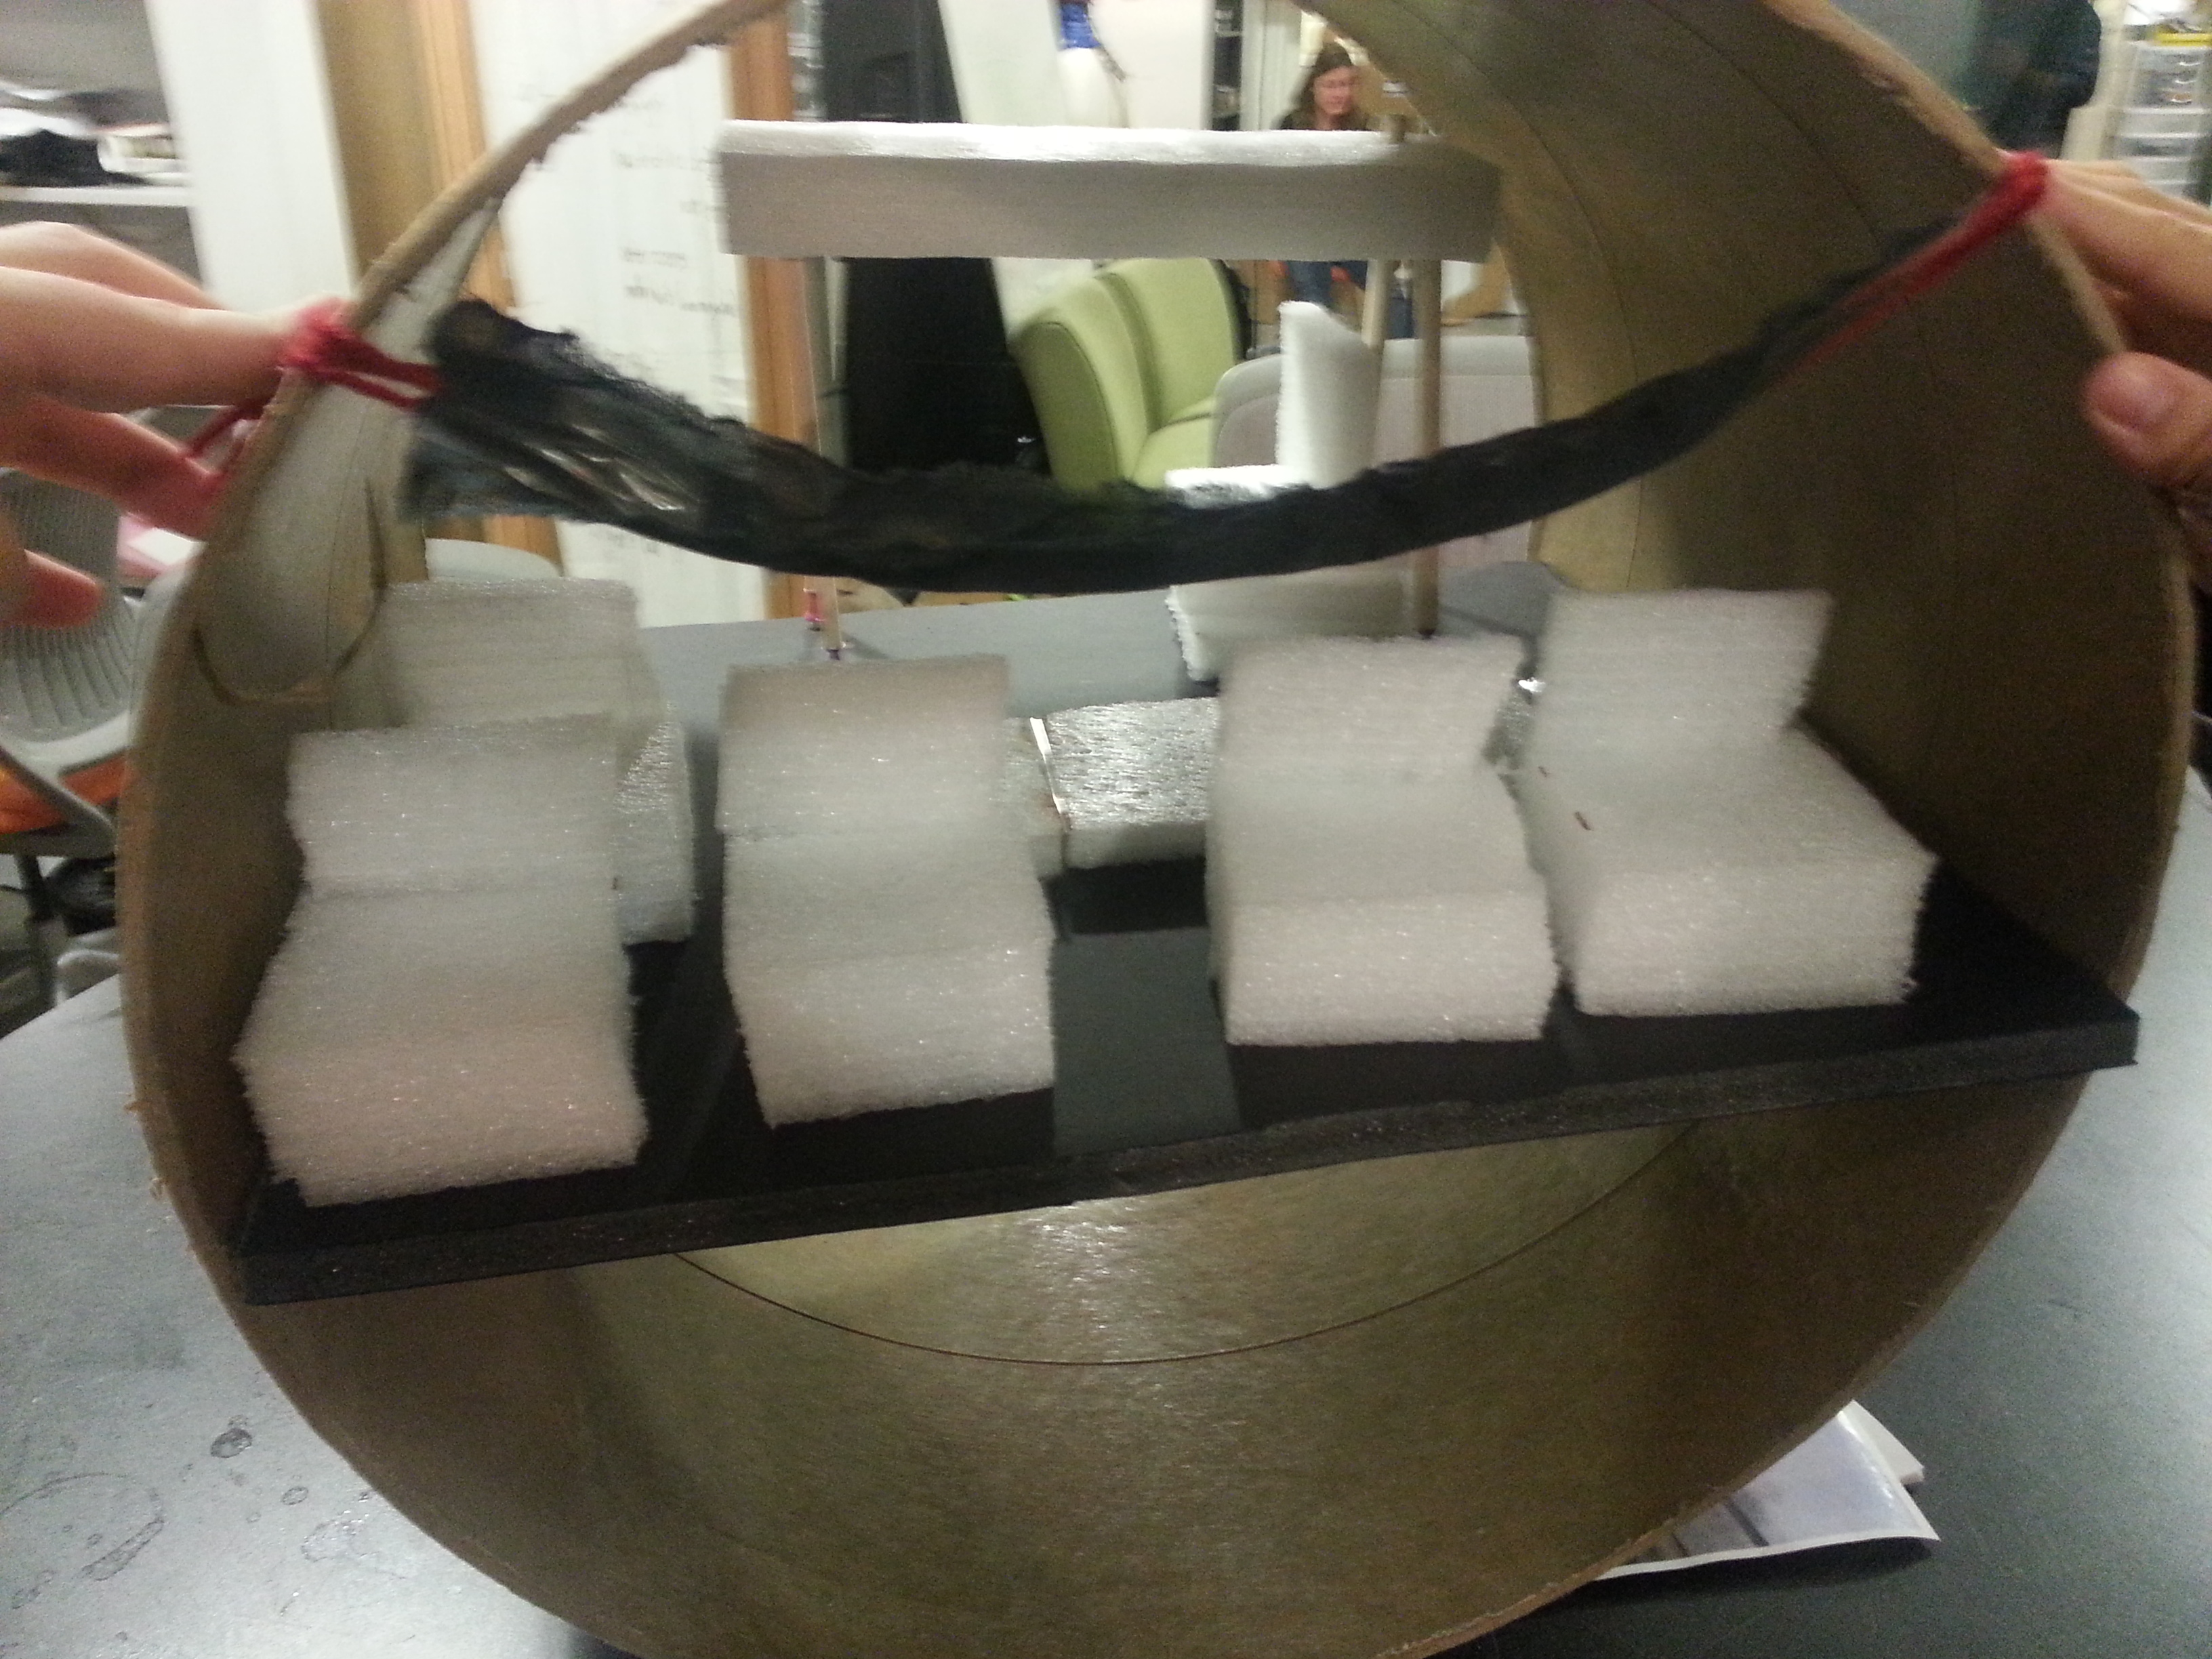
\includegraphics[width=7cm]{images/20140116_172733.jpg}
   \caption{Plane section dedicated to sleep and relaxation with two configurations: take-off/landing (left) and cruise (right)}
  \label{fig:20140116_172733}
\end{figure}

We also studied the possibility of using hammocks but the available space in the cabin was not sufficient to make it work.

\subsubsection*{Family Area}
When talking about passengers with reduced mobility people generally picture wheelchair users and passengers with other physical handicaps, but in a sense, families with young children and pregnant women also have reduced mobility compared to the average passenger. In order to address their specific needs our team designed an entire section of the plane to be the family compartment.

We designed this section to be flexible and easily adaptable to family needs. If parents want to sit close to their children and look after them they can get rid of the armrests and convert their row of seats into a sort of bench allowing the family to stay together during the flight. In order to make it easier for parents, children and pregnant women to move through this area we coupled our idea of a bench with the design of a retractable table that can be folded and unfolded between two consecutive rows of seats facing each other. When the table is unfolded it is then easier for people on the benches to access the aisle as shown on the following pictures. 

\begin{figure}[h]
  \centering
     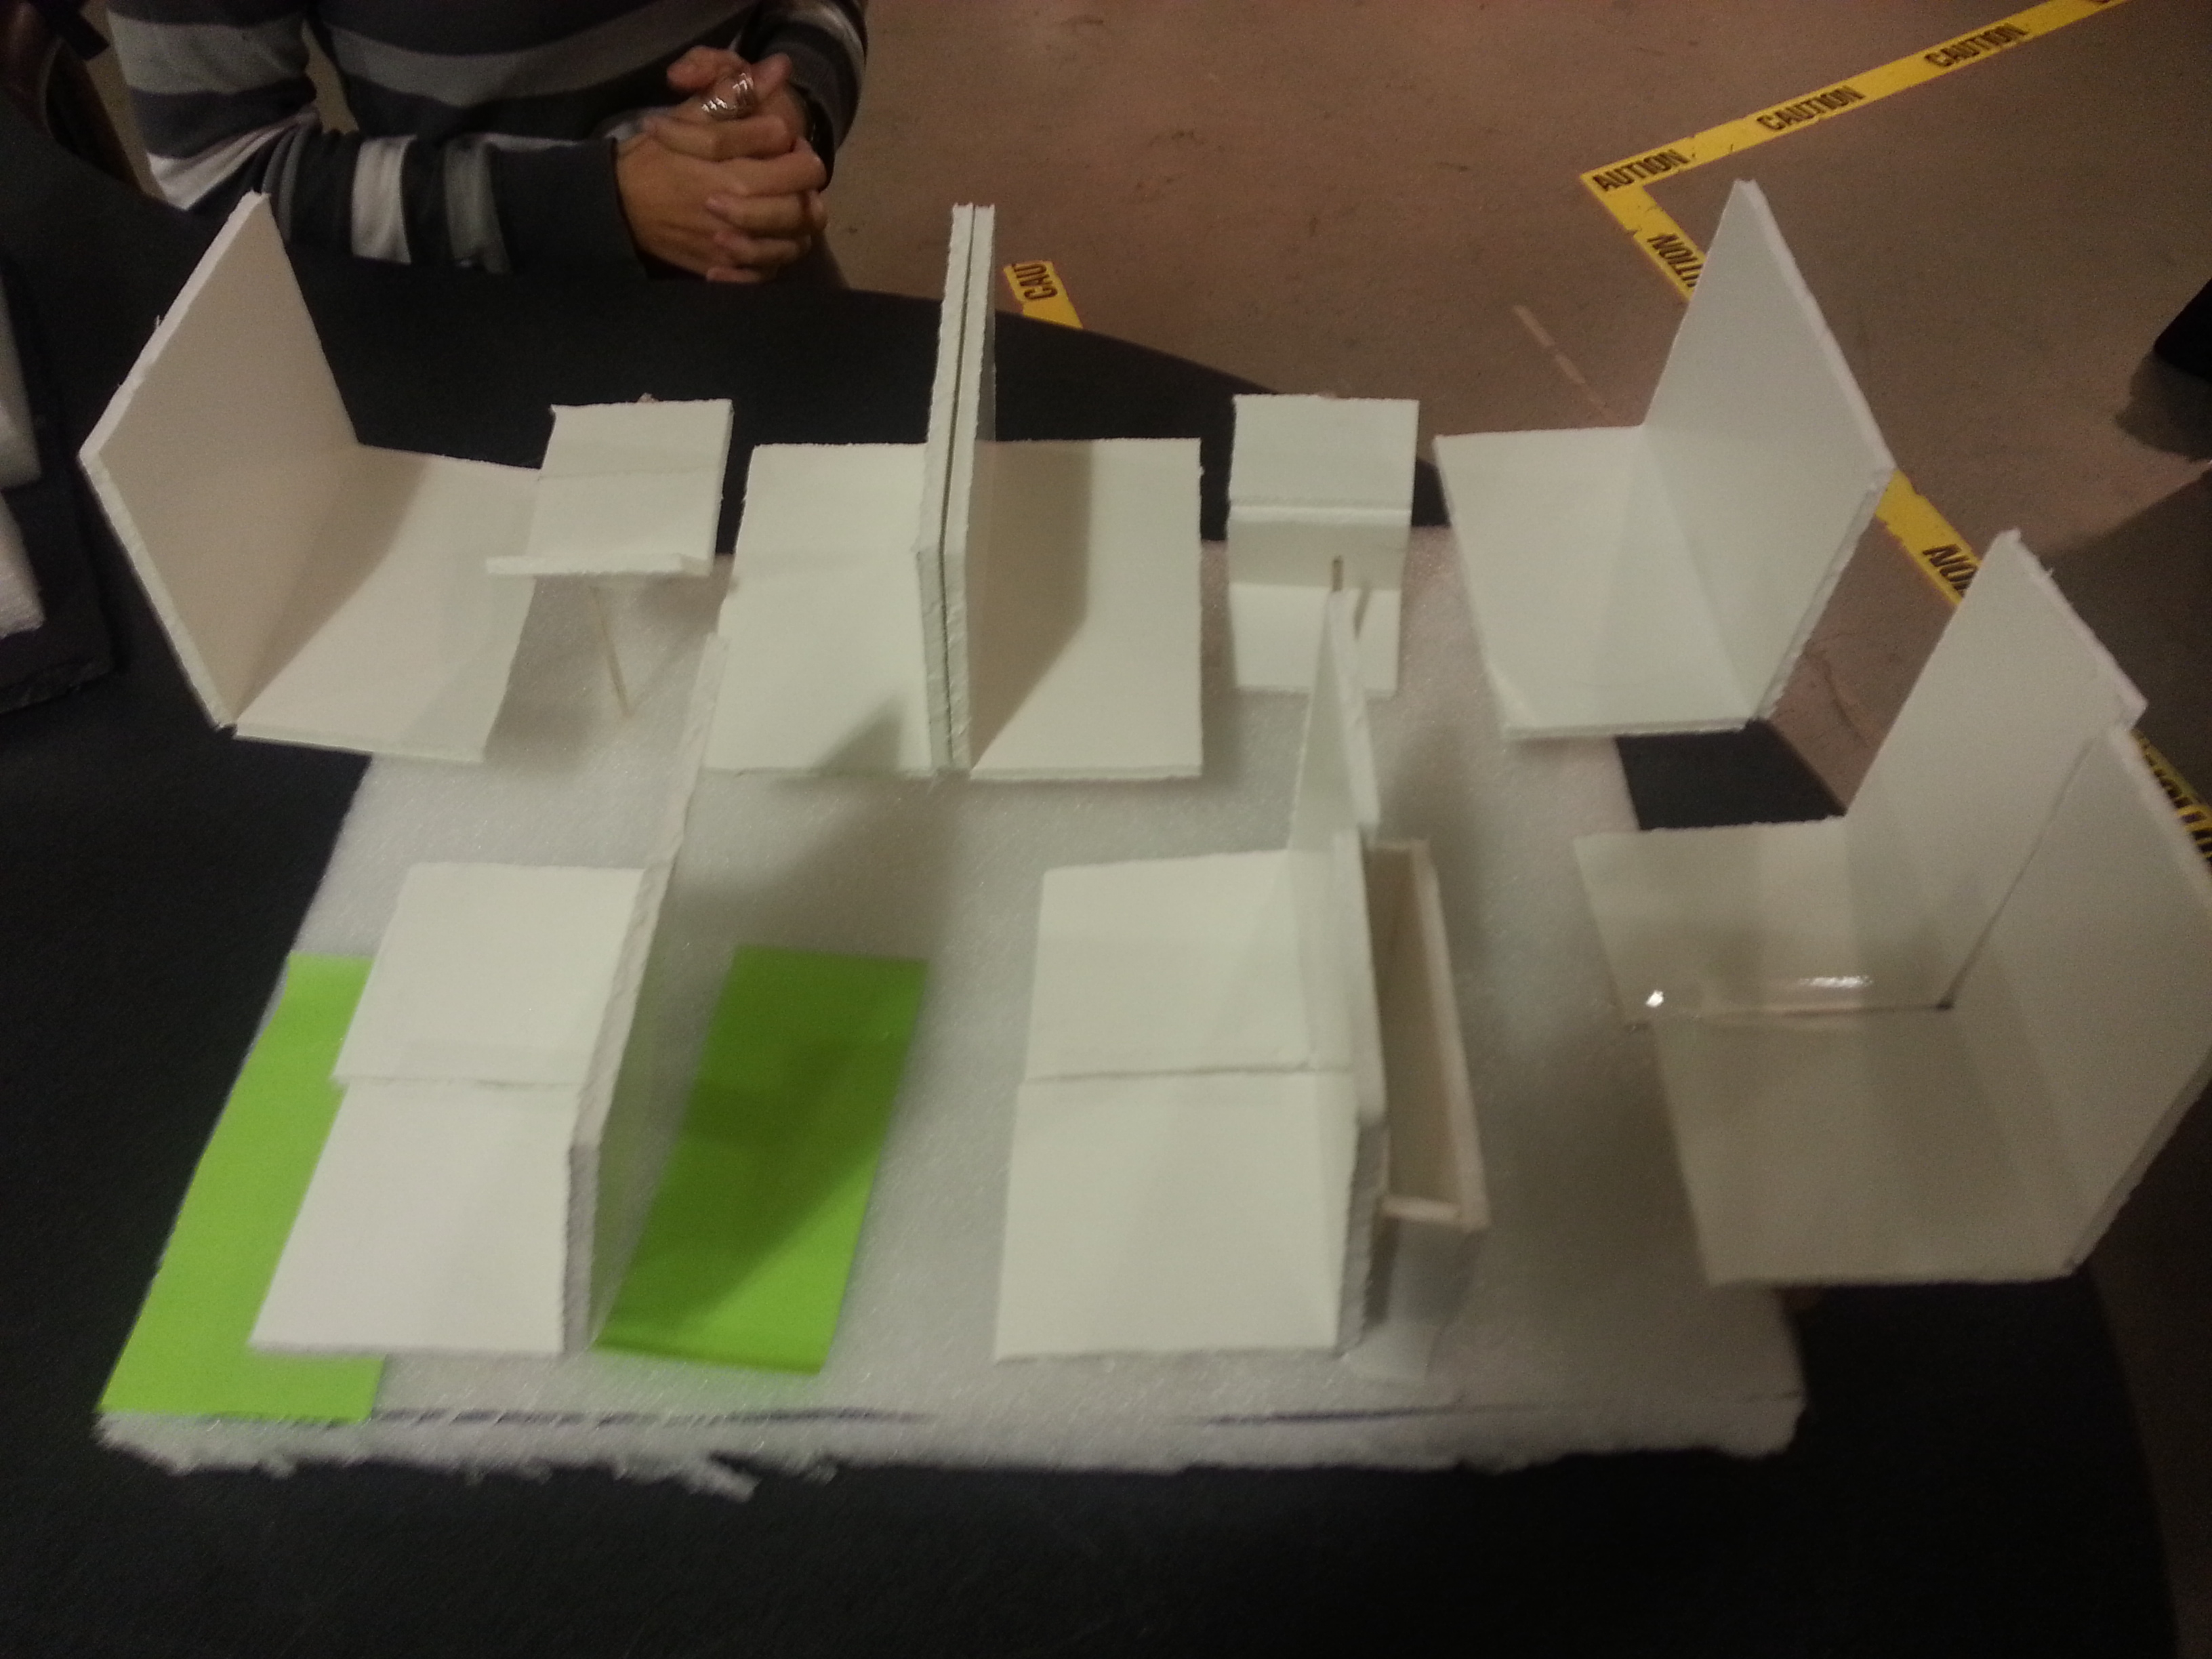
\includegraphics[width=7cm]{images/20140116_173112.jpg}
   \caption{Plane section dedicated to family with two configurations: take-off/landing (left) and cruise (right)}
  \label{fig:20140116_173112}
\end{figure}

We also considered the fact that the family section of the plane could be sound proof in order to prevent disturbances to the sleeping compartment and concentrate the noise of children playing together in one single area.

\subsubsection*{Gym Area}
When our team brainstormed about what people would like to do during their flight we thought that being able to move your limbs and stretch was a big issue, especially for people with blood circulation problems. In order to solve that we thought that having convertible seats that can be turned into yoga mats or that can be used as gym accessories could improve our user’s experience. We imagined a cabin layout that is standard for takeoff and landing but that can be turned into a gym area during the cruise, as displayed in the figures below. \\

\begin{figure}[h]
  \centering
     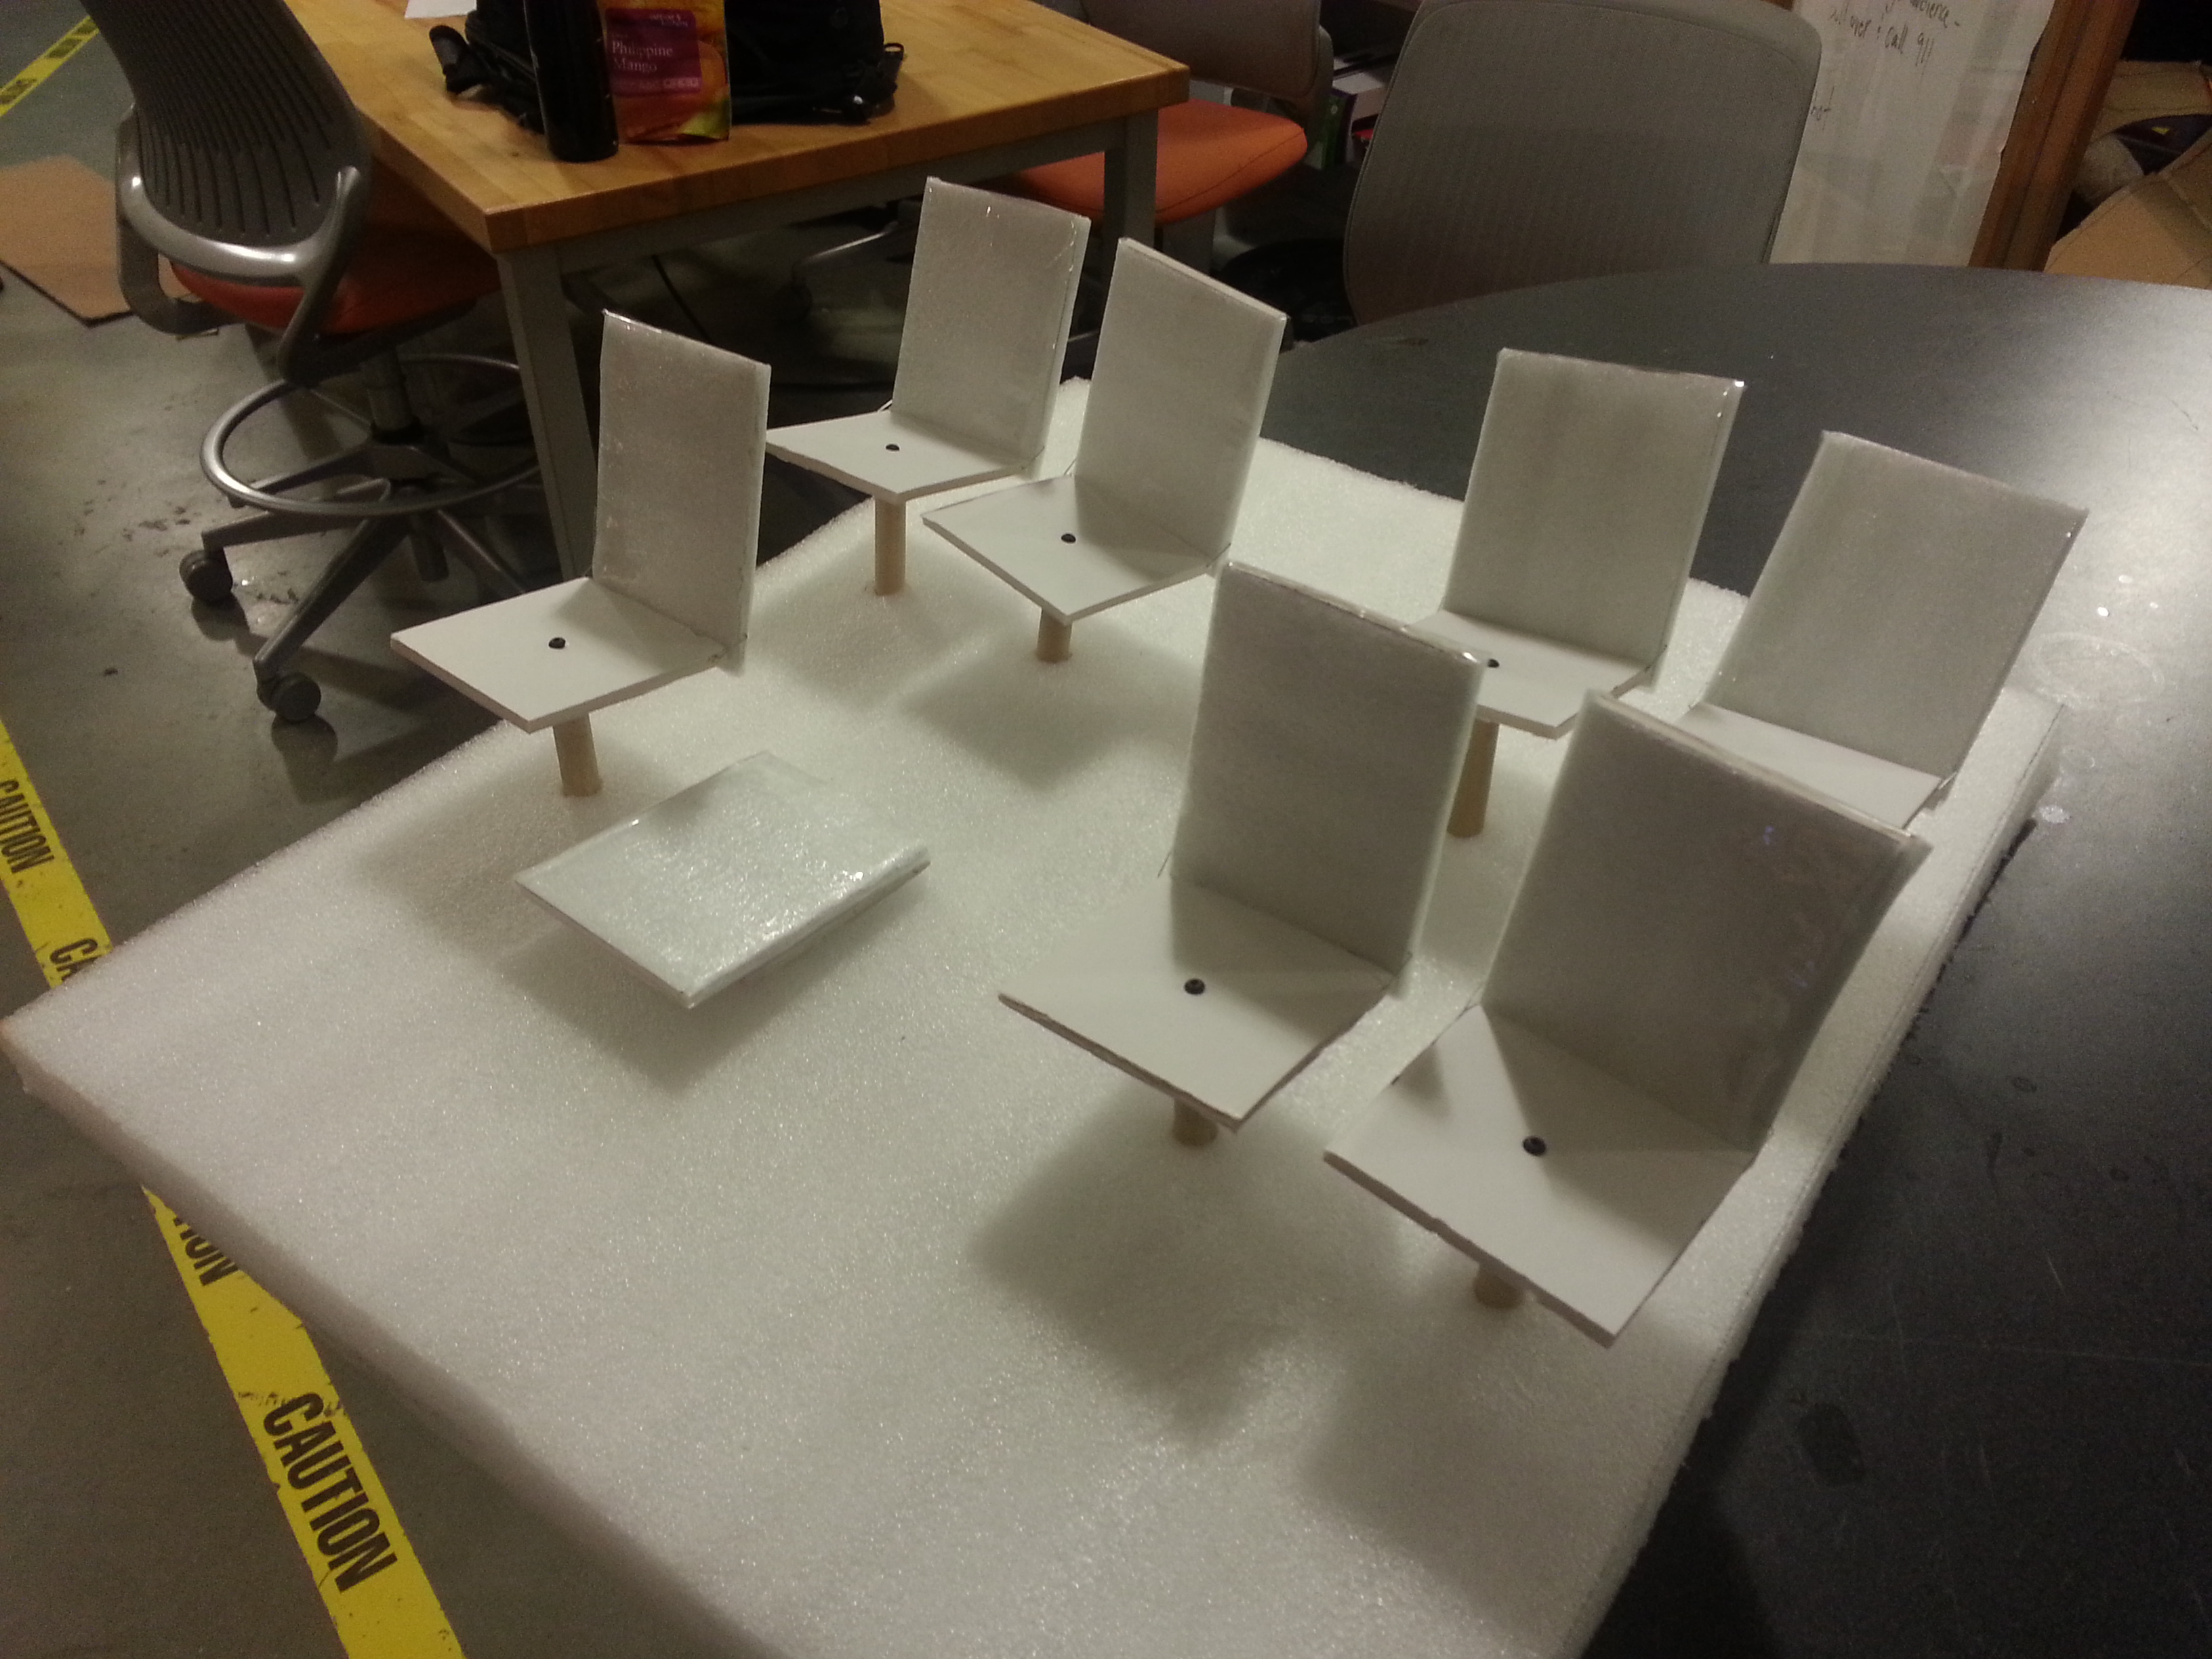
\includegraphics[width=7cm]{images/20140116_172402.jpg}
   \caption{Plane section dedicated to sports and physical training with two configurations: take-off/landing (left) and cruise (right)}
  \label{fig:20140116_172402}
\end{figure}

People with reduced mobility sometimes need to do physical therapy (PT) exercises to avoid blood circulation issues. However, handicapped people can rarely do their PT exercises alone so it’s possible that flight attends could be trained specifically to assist these passengers.

We also took into account the fact that people are often thirsty due to perspiration when they are physically active so we thought about a system of individual straws that would be available in each passenger’s space allowing to drink water whenever they want without having to call the flight attendants or move across the cabin. This idea can also be extended to all the sections and all the passengers allowing them to feel more in control and more independent.

\subsubsection*{Book Nook}
Since a lot of people, including those with reduced mobility, travel by plane for professional reasons our team wanted to design a plane section that imitates the cosy atmosphere of a coffee shop where people feel relaxed and comfortable while working.
To do so we imagined convertible seats that can be turned into couches and provide better support for people with reduced mobility. 

\begin{figure}[h]
  \centering
     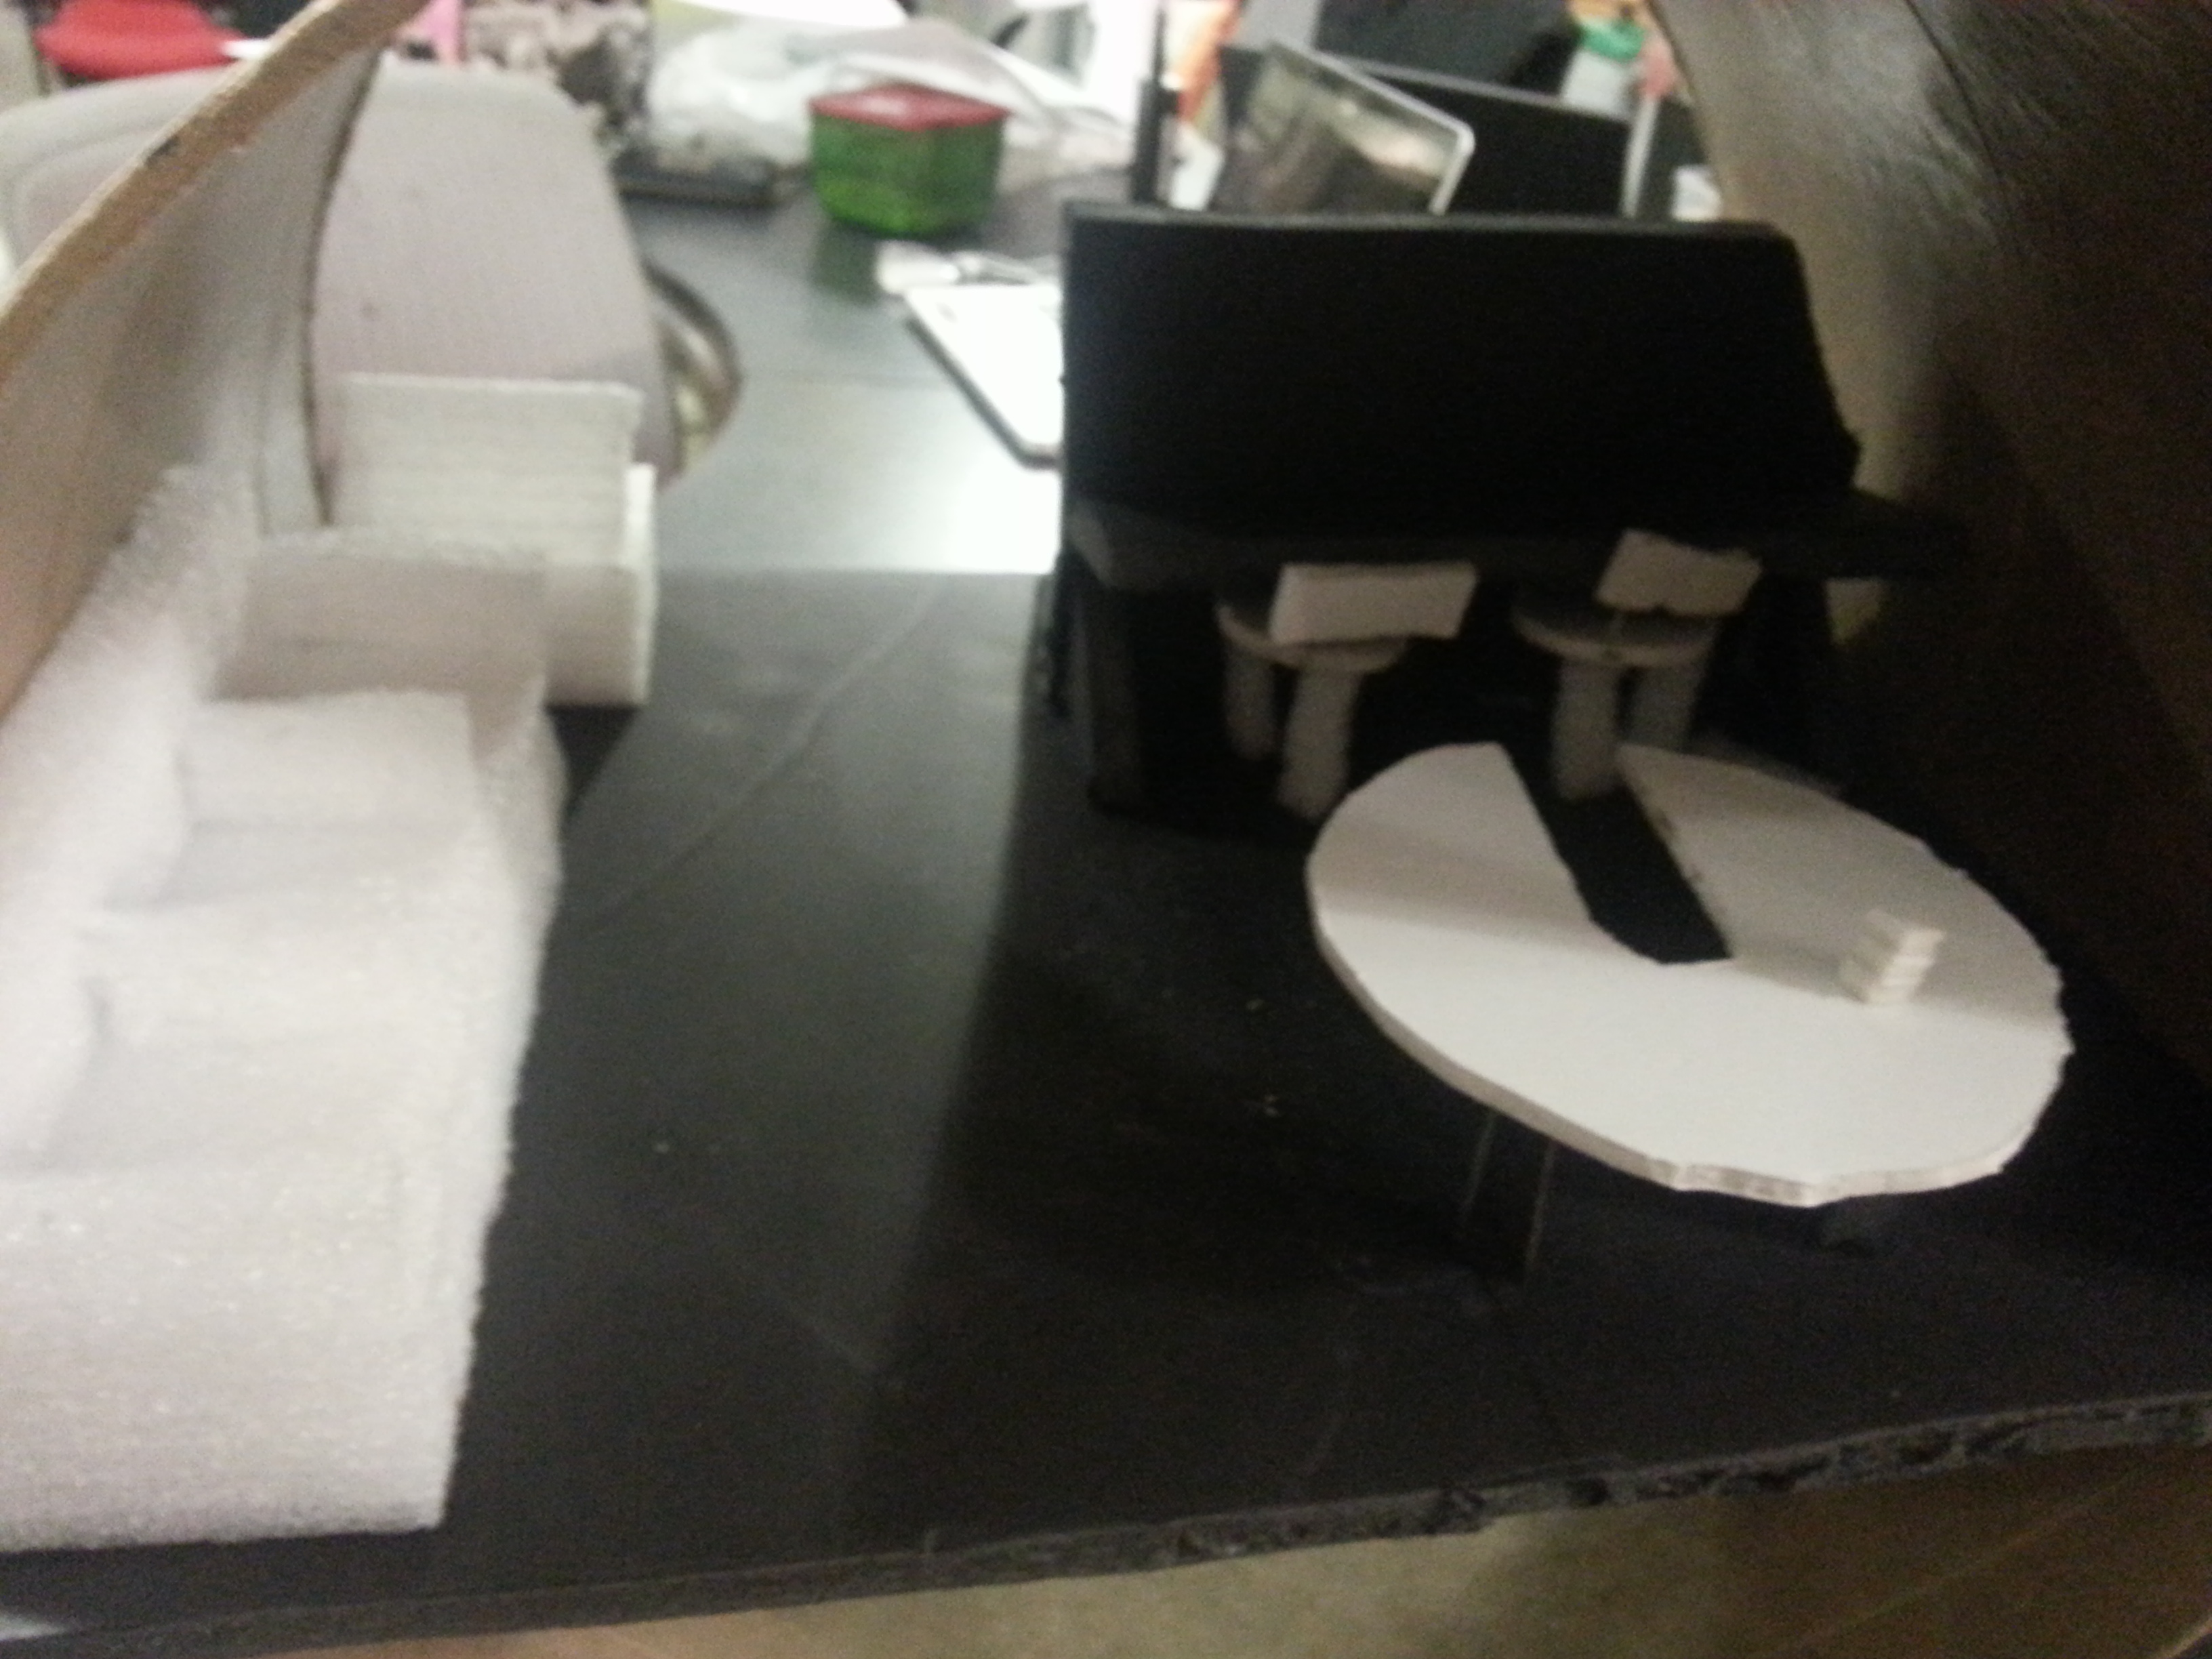
\includegraphics[width=7cm]{images/20140116_172928.jpg}
   \caption{Plane section dedicated to work in a cosy atmosphere with two configurations: take-off/landing (left) and cruise (right)}
  \label{fig:20140116_172928}
\end{figure}

We also thought that having a round table with one or two flight attendants in the center providing drinks was a good way to have them closer to passengers requiring more attention and assistance.

\subsubsection*{Ease of Access - Carousel}
We decided to fully dedicate the last plane section we designed to people with reduced mobility. In the previous sections we addressed their issues by trying to improve everyone experience so that handicapped people would not feel segregated, but for this last section we focused specifically on their needs and expectations. 
Our team found out that boarding and disembarking from the plane and moving in/out of their seats were the biggest issues for passengers with reduced mobility. In order to improve this part of their flight experience, our team decided to get rid of the current cabin layout where seats are lined up. 

We wanted to explore a different configuration where the seats are part of a carousel system that rotates so that any time a passenger enters the aircraft the seat right in front of them is empty. This would limit the distance people have to cover to get to their seat and should make it easier for them to move in/out of their seat since there is no obstacle in front of them as shown in the following pictures.

\begin{figure}[h]
  \centering
     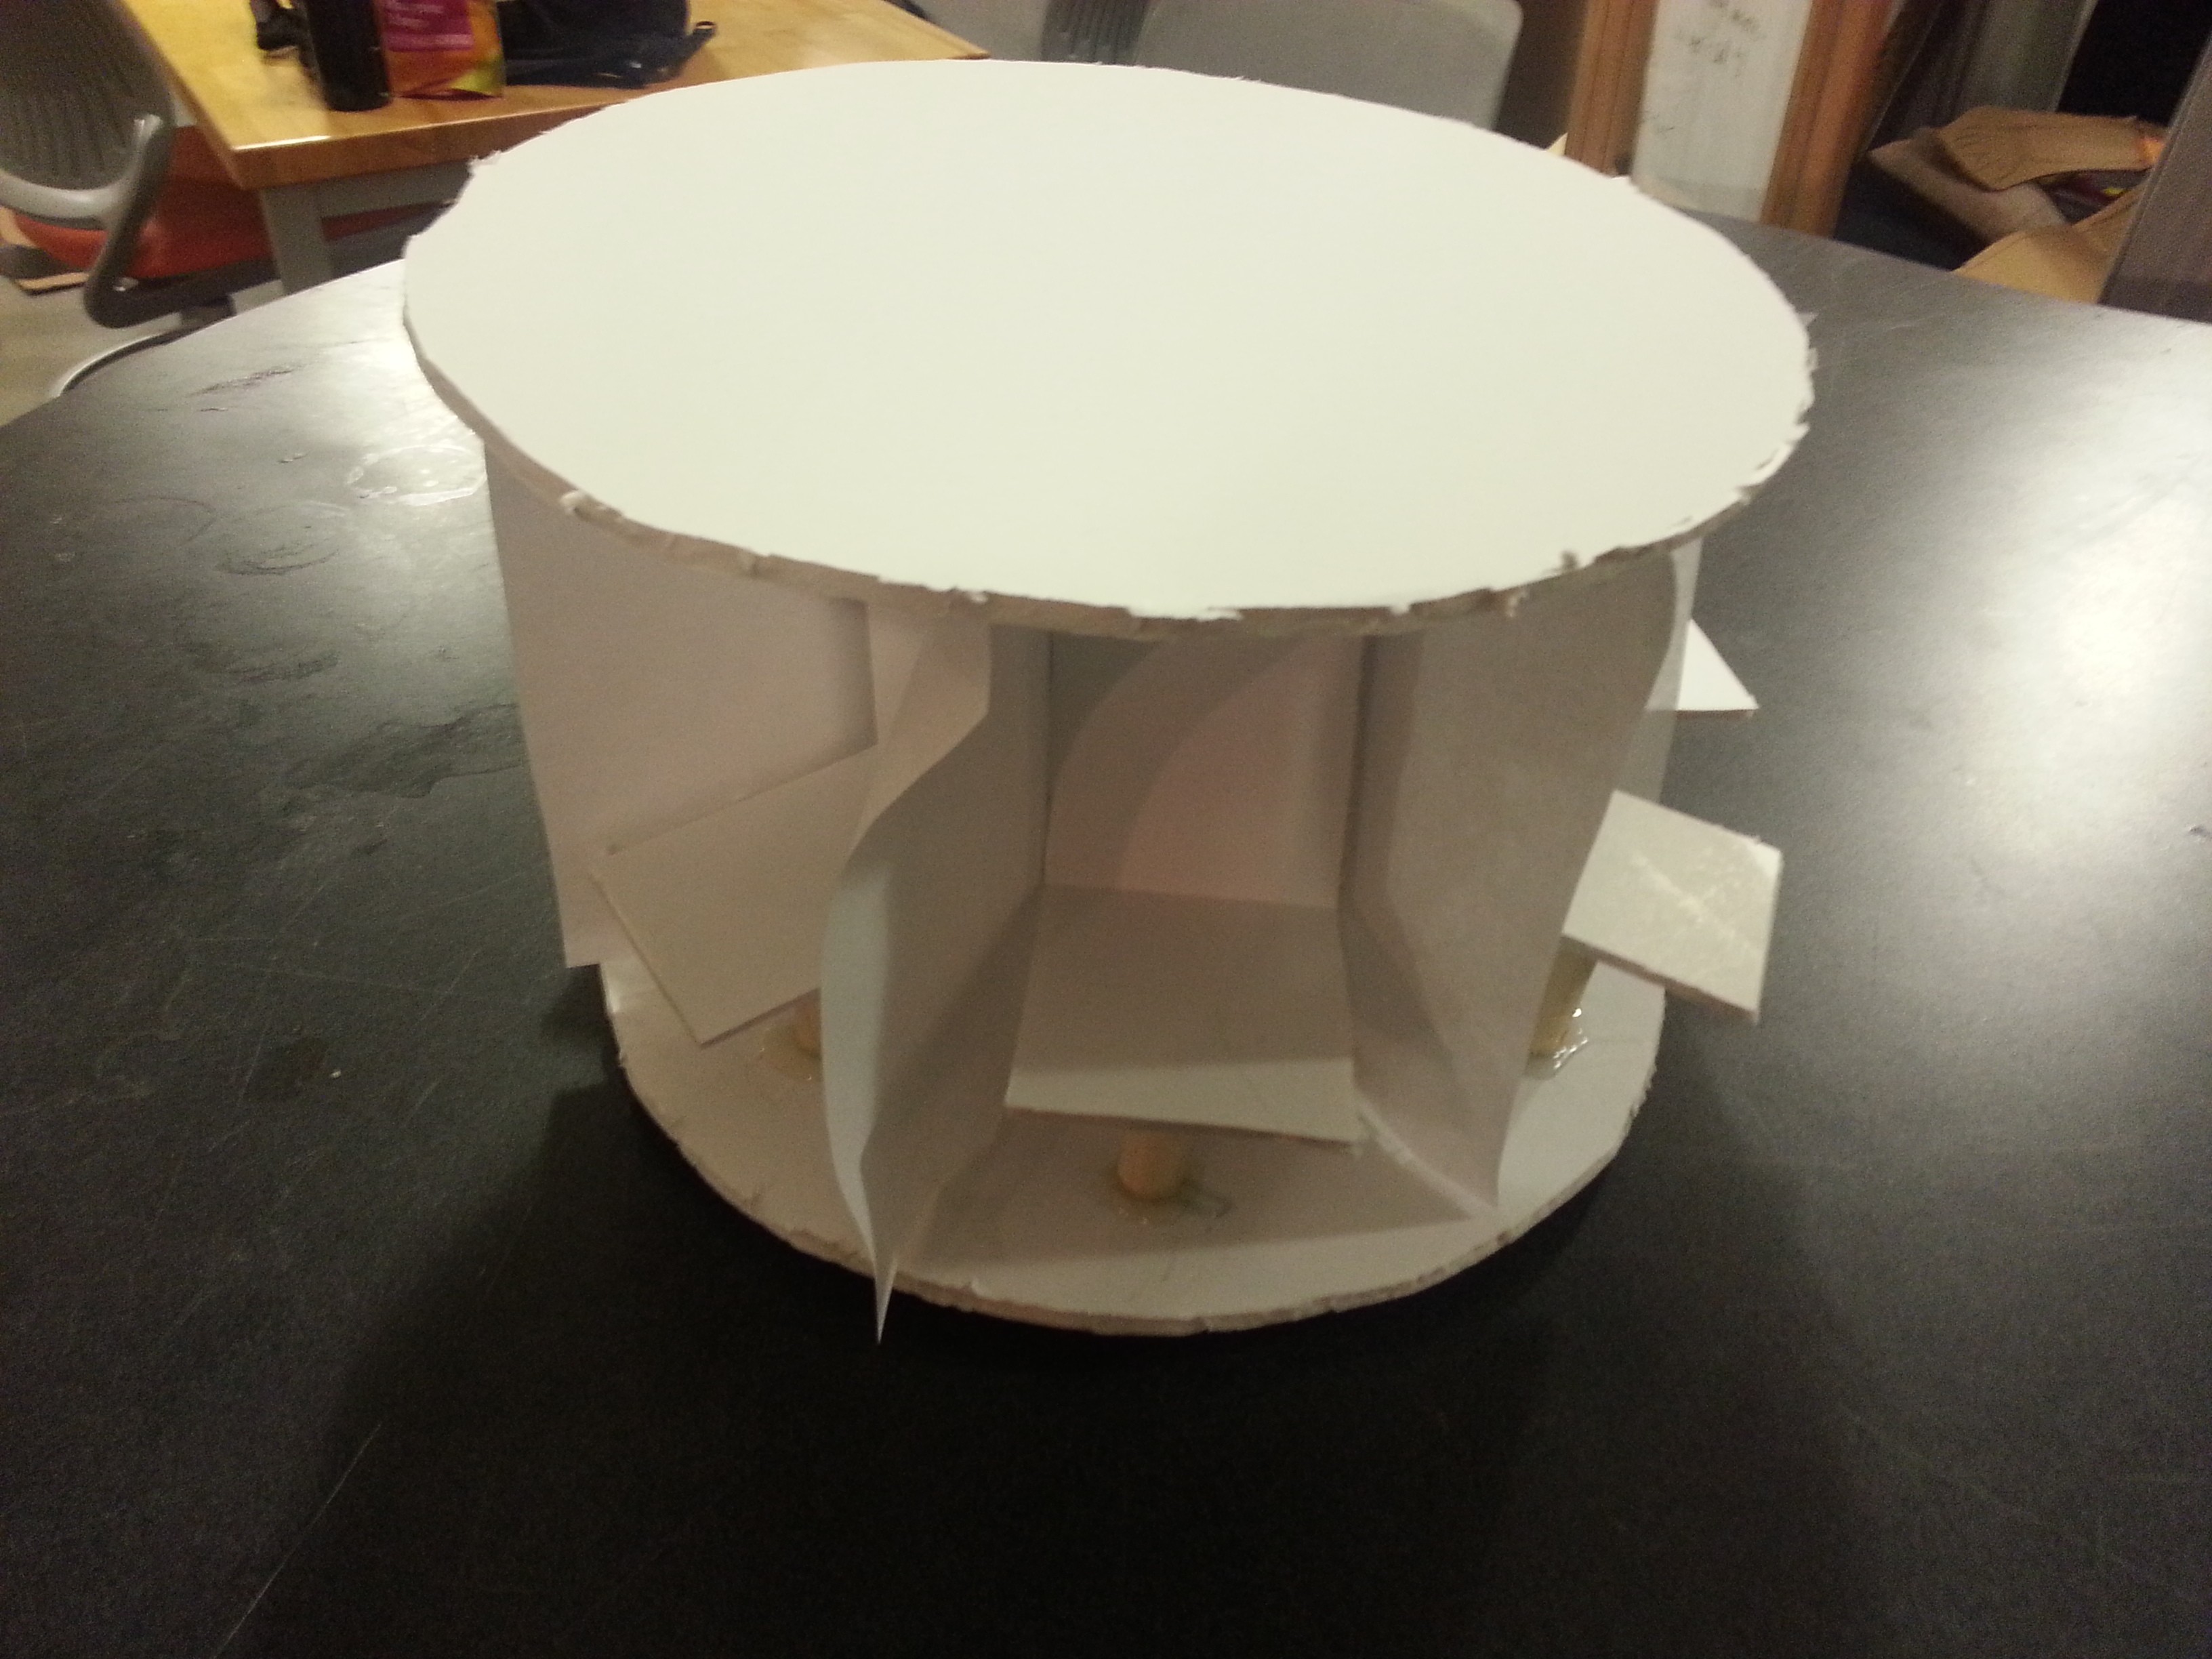
\includegraphics[width=7cm]{images/20140116_172516.jpg}
   \caption{Plane section dedicated to people who need easily accessible seats}
  \label{fig:20140116_172516}
\end{figure}

We also thought that one of the seats from the carousel could be removed from the circle, making the center of the system accessible. If the central part of the carousel can be accessed then it could be used as a place where wheelchairs or other equipment could be stored.


\subsubsection{Learnings}
\begin{enumerate}
	\item The following learnings came as a result of team discussions, analysis, and feedback from the teaching team. 
	\item It is difficult to reconfigure the cabin without losing seats. However, to maximize profit airlines do not want to lose any seats, making it important to maintain the same number.
	\item The number of possible cabin configurations increase with the implementation of dynamic seats.  Dynamic seats will allow for movement of cabin sections to meet the demands of each passenger. 
	\item Personalizing the flight would improve the experience for all passengers, not just disabled passengers. Many passengers compare the boarding and flight experience to the herding of cattle. By allowing passengers to choose their prefered cabin surrounding or configuration, they play a role in their experience and have more control over their situation. 
	\item Flight attendants may be able to play different roles in the passengers’ experiences.  They would be able to cater more toward what a passenger wants instead of performing a wide range of services for all passengers who might not need or want a certain service. 
	\item Every cabin configuration that can be implemented needs to have accessible features to fit the wide range of users our project encompasses.  The new cabin configurations cannot neglect our target user and should not make them feel singled out. 
\end{enumerate}

\subsection{Dark Horse Version 2}
\subsubsection{Benchmarking}
Our learnings from version 1 inspired us to continue to explore changing the cabin layout while also putting additional emphasis into the boarding process. We realized that if we could make the seats more accessible, we would be able to alleviate some of the pain brought on by the transfer process into today’s chairs. We looked at cabin configurations like the one in Figure \ref{fig:cabin_against_wall.jpg} where the seats face toward the inside of the cabin as opposed to the front. By having the seat face the passenger, it would be much easier to get in without having to worry about climbing over armrests or other passengers. 

\begin{figure}[h]
  \centering
     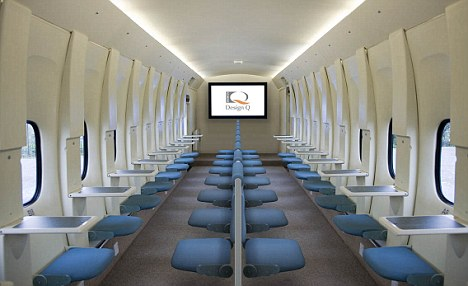
\includegraphics[width=7cm]{images/cabin_against_wall.jpg}
   \caption{Vertical seating being designed for airplane chairs. Source: http://www.dailymail.co.uk/news/article-1215081/Packed-like-sardines-New-aircraft-design-plans-seat-passengers-face-face.html}
  \label{fig:cabin_against_wall.jpg}
\end{figure} 

The team researched this further and found that seats are configured to be faced either toward the front or back for safety reasons relating to the forces that passengers could experience during flight. Having seats face inward could subject passengers to excessive lateral forces. Additionally, from the public reception of the configuration shown in Figure \ref{fig:cabin_against_wall.jpg},  we found that passengers would not feel comfortable directly facing other passengers. Thus, we looked at different types of boarding mechanisms that would enable a simpler boarding experience but that would also retain the safety level found in airplanes today. 

\subsubsection{Description of the prototype}
In order to solve the problems faced by mobility challenged passengers we tried to radically change the boarding experience for everyone. To this end, our team decided to further investigate carousel concept developed in dark horse version 1 and push it to the extreme.

In order to go as far as possible with this concept we decided to:

 \begin{easylist}[itemize]

& Rethink the whole boarding process from the gate to the seat by creating a carousel inspired by a conveyor belt system through the entire plane.

& Design for an extreme case: a person with no mobility, i.e. a passenger without the use of any limbs. It made our mission more challenging but we thought it could be a good way to make sure we do not overestimate what a people with reduced mobility can or cannot do. In order to reach our goal, we brought a new persona: a mannequin filled with sand to mimic the weight of a real person.

\end{easylist}

We wanted our new persona to go through all the steps of the brand new boarding process we imagined:

\begin{easylist}[itemize]

& Waiting in line at the airport gate where position in the line is determined by seat number. This will facilitate the boarding process since people will have to board in the order defined by the cabin layout. Those in the aft of the plane would go first.

& While waiting, our new persona would be transferred to an airport chair that will then facilitate the transfer to the seat.

& When boarding starts, our persona will use a transfer mechanism located in the front of the cabin to reach his or her seat. Here are different options we modeled:

 \begin{easylist}[itemize]
	& The \textbf{hammock}-type transfer involves a seat that is detachable and can be moved from one chair to another using a lift
\begin{figure}[h]
  \centering
     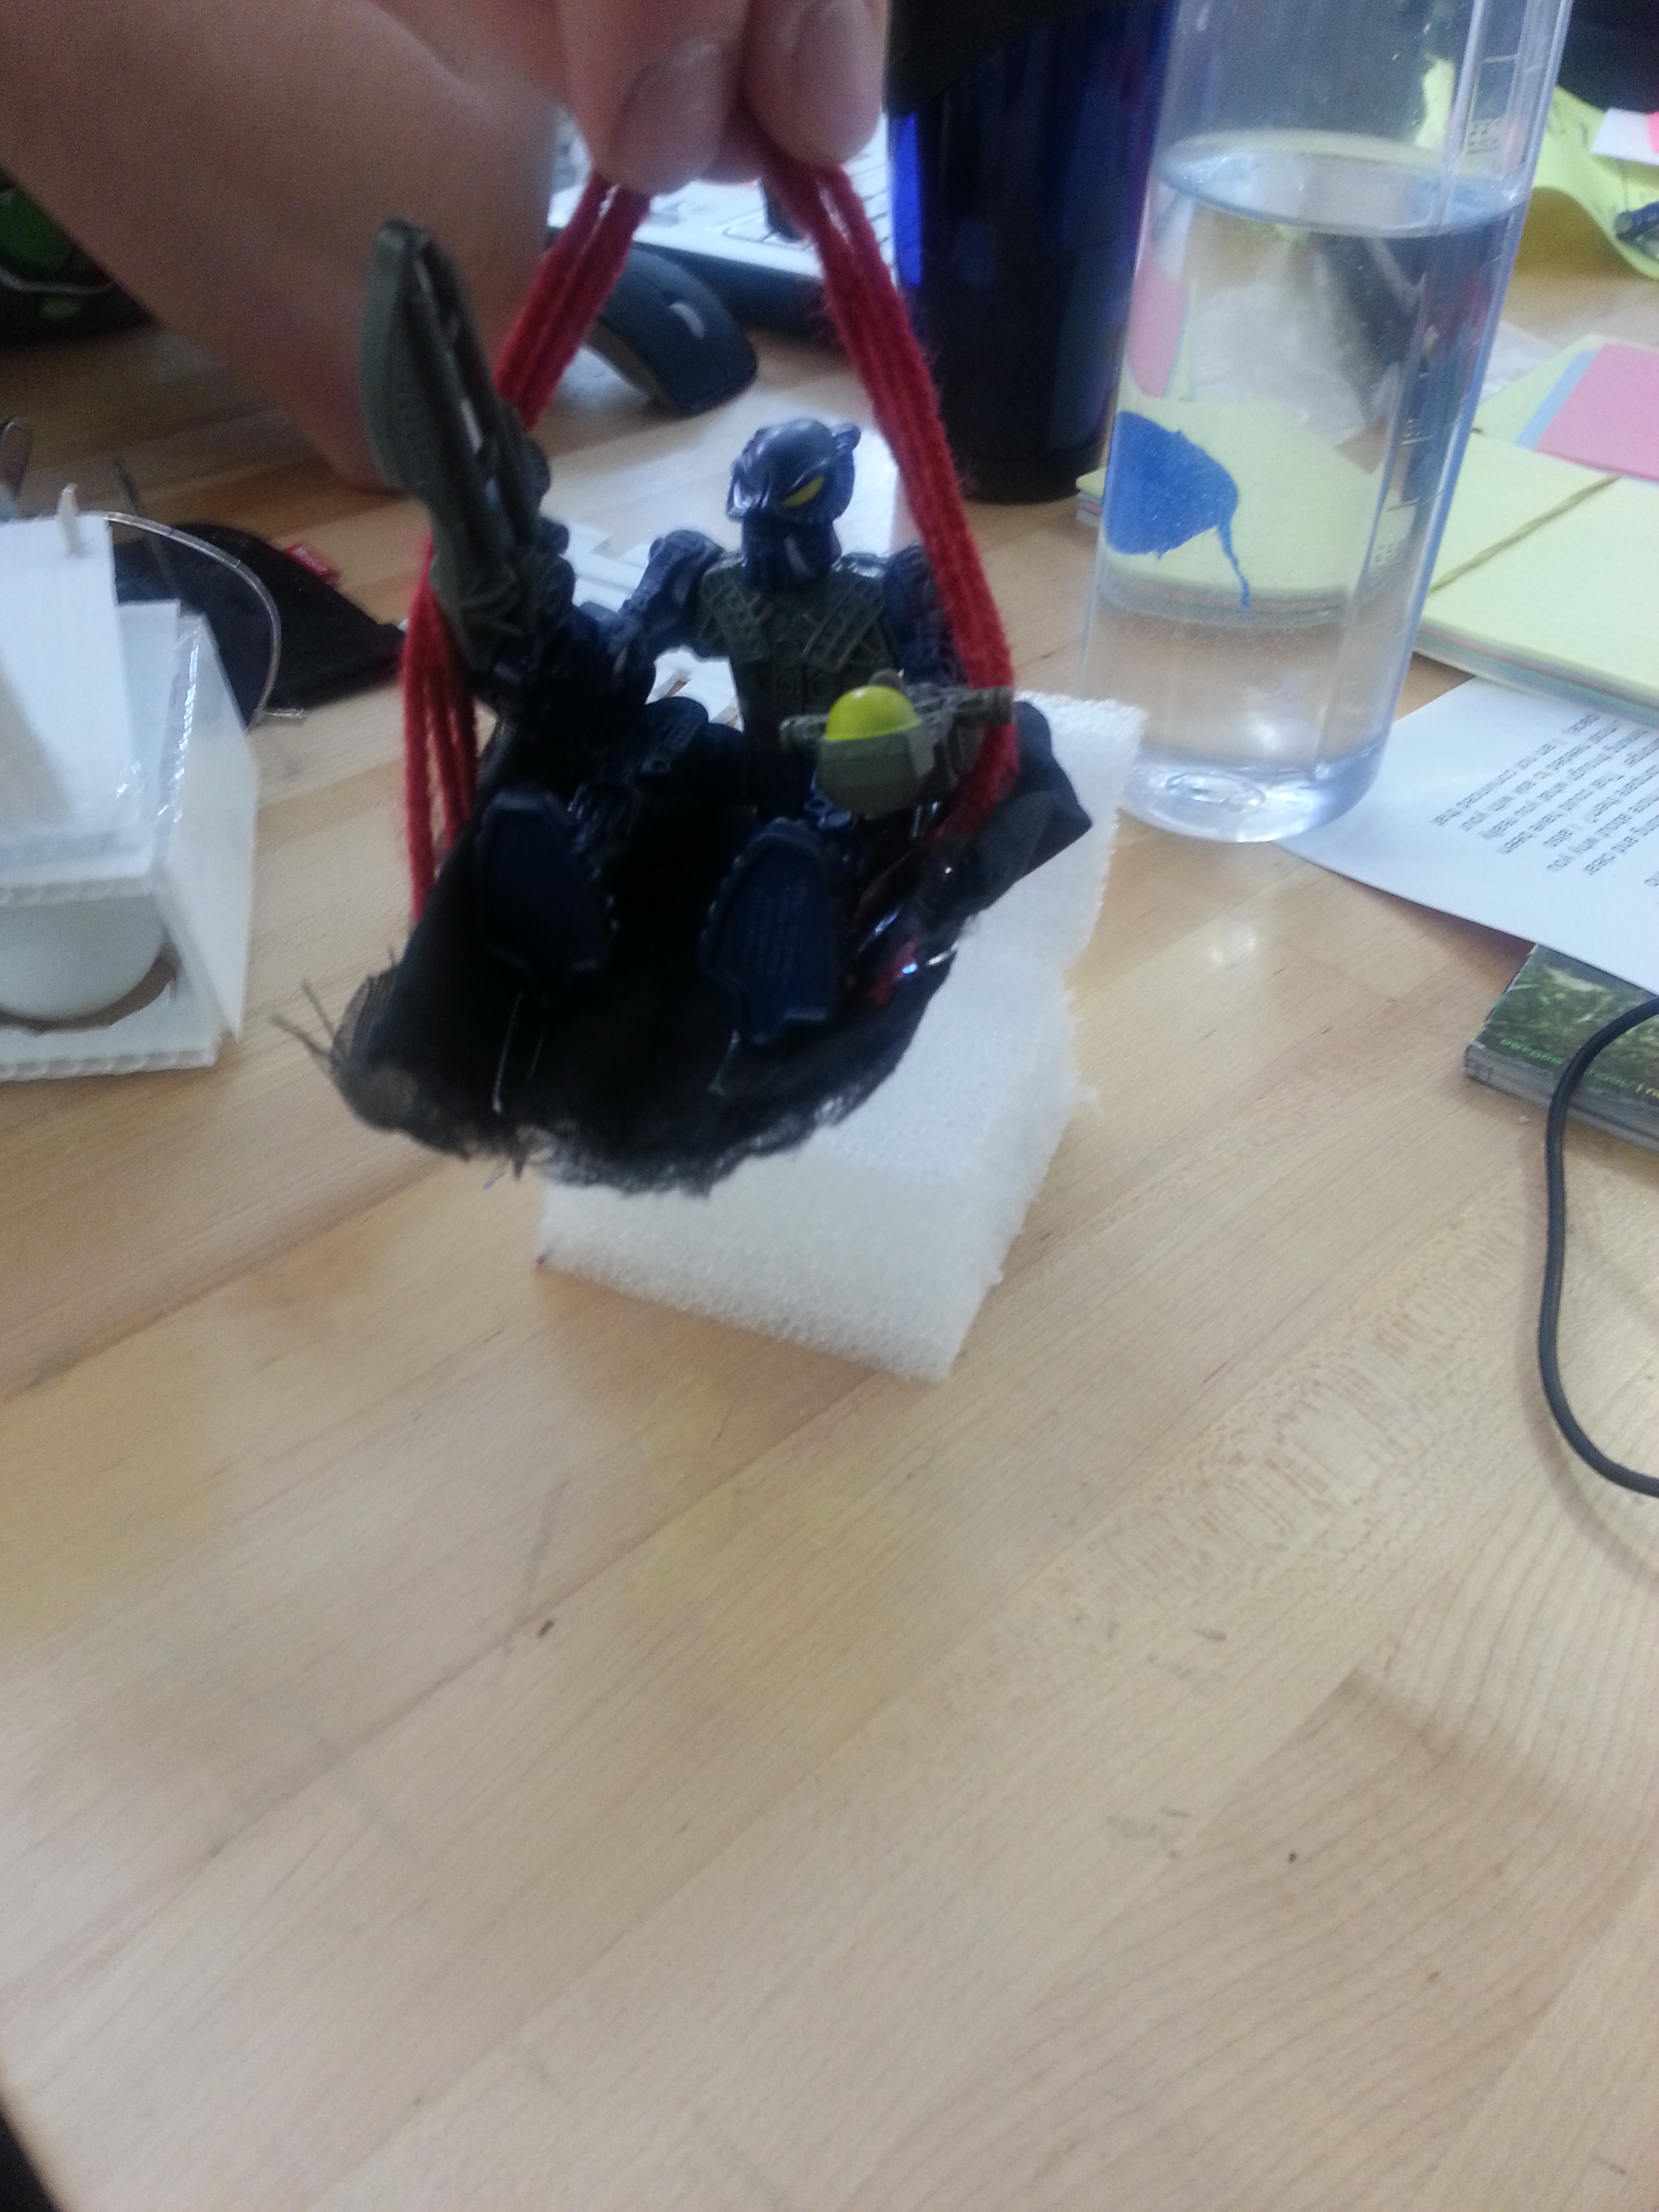
\includegraphics[width=7cm]{images/20140120_121827.jpg}
   \caption{Hammock transfer to enable people to go from the airport chair to their seat}
  \label{fig:20140120_121827}
\end{figure} 

	& The \textbf{comb} seat involves two separate pieces which have interlocking teeth; one can be lifted up, bringing the passenger with it, then installed on another chair
\begin{figure}[h]
  \centering
     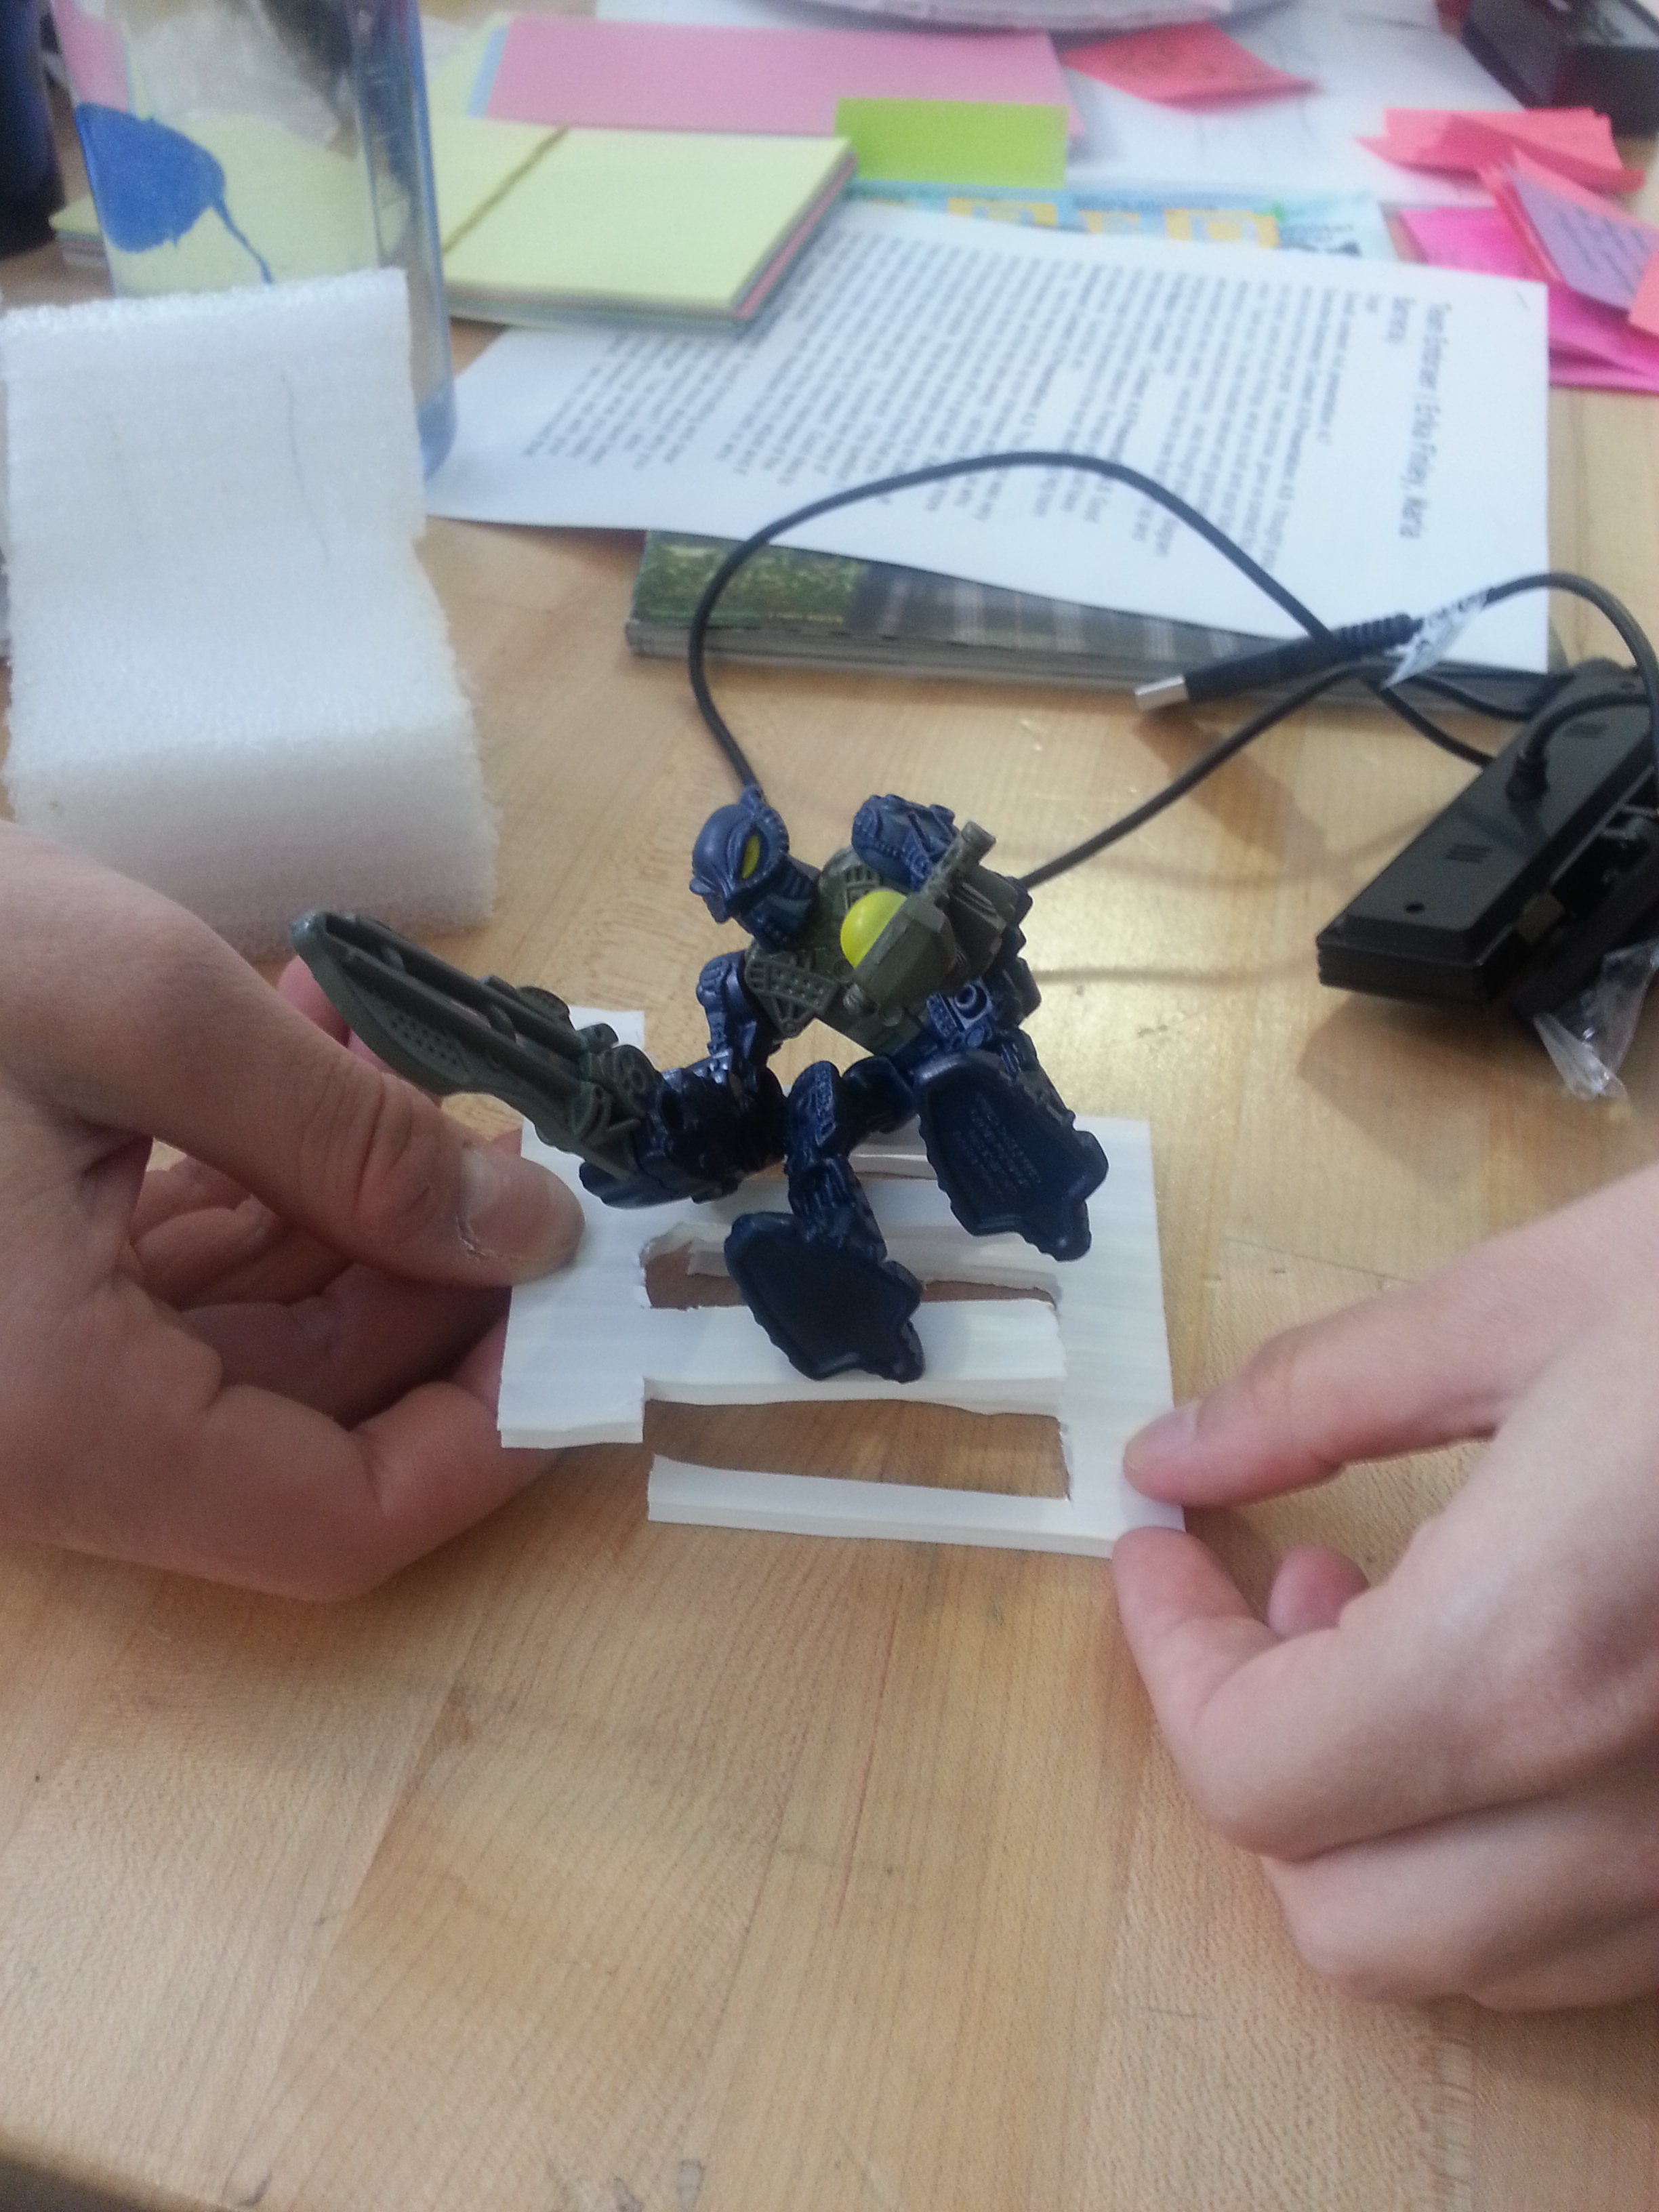
\includegraphics[width=7cm]{images/20140120_121849.jpg}
   \caption{Comb seats that would facilitate the transfer from the airport chair to the seat}
  \label{fig:20140120_121849}
\end{figure} 

\end{easylist}

& Once our user is seated, his seat will then be moved via the carousel/conveyor belt to its standard position as shown on the next drawing.

\begin{figure}[h]
  \centering
     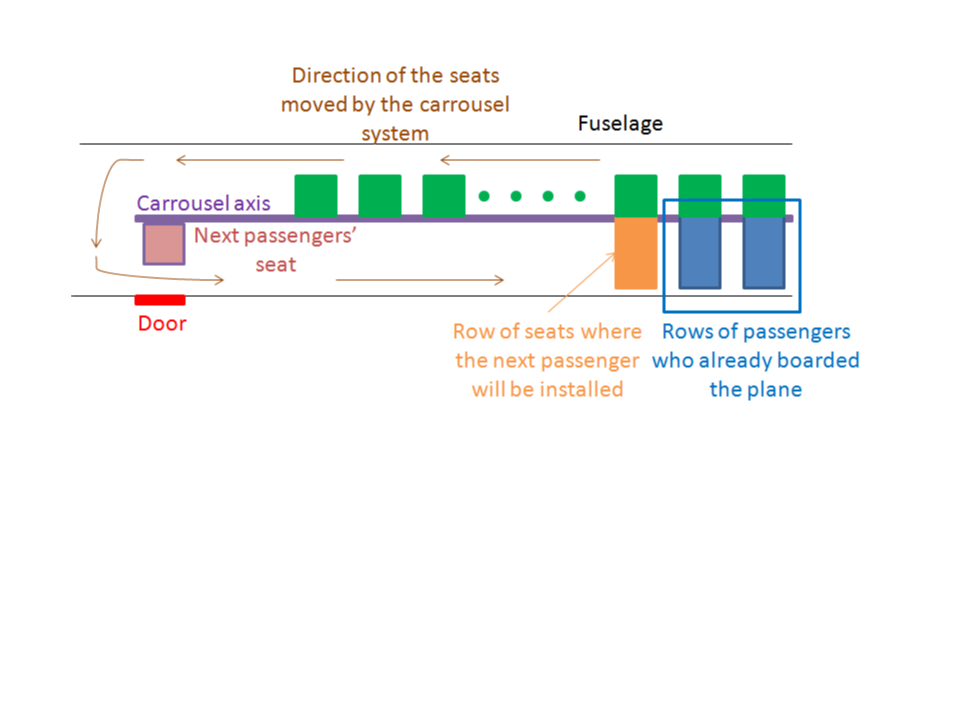
\includegraphics[width=7cm]{images/carousel_for_the_dummies.png}
   \caption{Carousel system conveying the seats from the entrance of the plane to their appropriate location}
  \label{fig:Carousel_system}
\end{figure} 
\end{easylist}

\subsubsection{Learnings}
The learnings for this iteration of darkhorse resulted from team discussions, user suggestions and feedback, observations of the user persona, and teaching team feedback. \\

\begin{easylist}[itemize]
	& The transfer mechanism to move the user into the airplane chair is still a problem that needs to be addressed. The user has to be able to make it from the waiting lounge to the airplane seat with the feelings of control, comfort and stability. 
	& The experience prototype of boarding did not include a mechanism to deal with luggage. The process of storing and carrying luggage needs to be addressed within the prototype to represent the entire experience. 
	& Communication is key to allow our users to feel comfort, safe, and stable within the new process. The process needs to be communicated effectively and sufficiently to allow for our users to have a better experience and to feel as if this process is better than the previous boarding process. 
	& Users want to be able to worry and stress less about getting to their seats and finding a place for their luggage. The new boarding process would allow the users to use the boarding time on a more enjoyable pastime. 
	& The users have to exert less effort with this boarding process because boarding is automated and does not require the need to locate their seats and maneuver the aisle. 
	& Our user was concerned with bumping into objects or other seats or hitting the wall during movement. The boarding process needs to be done in such a way that the users and passengers feel safe and secure with the movement and with process as a whole.  Lateral accelerations need to be considered to create a smooth ride and efficient boarding process. 
	& Sensors would need to be implemented into a functional prototype or a mechanical prototype to simulate the actual boarding process by having the interim stops to board new passengers.  Sensors would also need to be implemented into the process to prevent collisions or accidents in the case of a malfunction. 
\end{easylist}

\newpage

\subsection{USP Dark Horse Prototype}
\subsubsection{Ideation}
Before starting our brainstorming sessions, we focused on defining the most critical issues based on our need finding research. As a result we emphasized the following three issues: \\

\emph{Broken Wheelchair}\\ This is one of the most notorious issues faced by wheelchair users. To understand the dimension of this problem, Channel 4 made an interview with a wheelchair and pointed out that his wheelchair had been damaged on four out of eight flights he took. This is quite critical, especially when we take in that wheelchairs represent independence outside the plane for them and that this mishandling causes a great deal of anxiety on them during the flight.  \\
 
\begin{figure}[h]
\centering
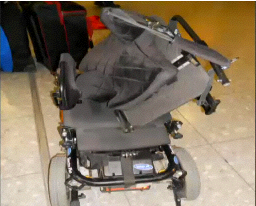
\includegraphics[width=7cm]{brazil_images/image001.png}
\caption{Broken wheelchair - Unknown user}
\label{fig:broken_wheelchair}
\end{figure}


\emph{Small Pitch}\\
 The small space between rows of seats is not a novelty to anybody who has already been on a commercial airplane. For people with reduced mobility the small pitch represents an increase of one’s limitation and a growing feeling that one is bothering other people. One feels like a sardine in a can, unable to get in/out of one’s seat.\\

\begin{figure}[h]
\centering
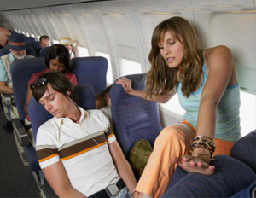
\includegraphics[width=7cm]{brazil_images/image002.png}
\caption{Characterization of the small pitch \cite{aislehumor}}
\label{fig:characterization}
\end{figure}

\newpage

\emph{Inaccessible WC’s}\\
 The inaccessibility of lavatories is another important issue that people with reduced mobility travelling on airplanes have to face. As our field research showed, people with reduced mobility take extreme measures to avoid going to the airplane lavatory because they are so tiny that they most of the times aren’t able to transfer themselves to the toiled seat and enjoy some privacy while inside it. As a result, users feel dependent on others.\\


\subsubsection{Dark Horse Candidates}
The following Dark Horse ideas were generated during our brainstorming sessions:\\

\noindent\emph{Mobile restroom}\\
The basic idea here is having a portable lavatory that can move closer to the user eliminating the difficult process of walking to the W.C., providing the user with autonomy. Nevertheless, as we thought further on the idea and asked other people about their impressions, we noticed that it was highly controversial because it would be very difficult to deal with hygiene, privacy and odors. Any failure on the mechanism would be catastrophic.\\

\noindent\emph{Modular Boarding}\\
 It consists of a mechanism similar to one of a rollercoaster. For this idea the group discussed two different forms to operate. On the first one, the plane would be just an exoskeleton receiving all the seats together; on the second one, each seat would individually be transferred from the boarding area to the interior of the plane. This solution eliminates the space constraint issue by allowing passengers to board outside of the plane and at the same time makes the boarding/exiting process faster. However, this solution would require changes in airports and increase of the airplane’s weight. Lastly, because this solution would have a similar mechanism as our CFP, we discarded it as it would generate less significant insights.\\

\noindent\emph{Rotating Access Seats for WCs}\\ It is a rotating seat on the lavatory’s wall to aid reduced mobility passengers to access the W.C. It provides maneuver space for the user to be transferred to the lavatory without increasing its size and improves privacy by allowing wheelchair users to close the door. It is a universal solution because it does not segregate a lavatory for specific users. On the other hand, this idea would increase weight and we still did not know how the user would react while using the mechanism. This idea was chosen to be the Dark Horse project.\\

\subsubsection{Benchmarking}

Our vision for what we wanted to accomplish with our Dark Horse prototype led us to examine different types of lavatory both accessible or not and being part of an airplane or not.  Considering this aspects we achieve the following research:

\noindent\emph{Current Airplane Lavatory}\\ By studying the current W.C. we were able to recognize the most critical aspects of the imperfections of the lavatory such as the space to maneuver and, related to that, the lack of privacy once it is necessary to let the door open for the aisle chair.

\begin{figure}[h]
\centering
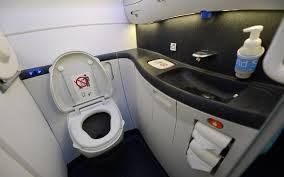
\includegraphics[width=7cm]{brazil_images/image012.jpg}
\caption{Current toilet on the airplane \cite{travel2012heard}}
\label{fig:current_toilet}
\end{figure}

\noindent\emph{Accessible lavatory}\\ By analyzing an accessible non-airplane lavatory we were able to understand the needs, concerning the bathroom, of people with reduced mobility and get to know the adaptations that exists nowadays.

\begin{figure}[h]
\centering
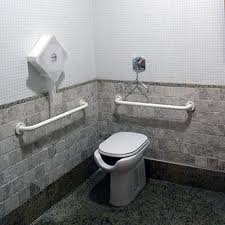
\includegraphics[width=7cm]{brazil_images/image013.jpg}
\caption{Accessible lavatory \cite{accessiblelav}}
\label{fig:accessible_lavatory}
\end{figure}


It is possible to observe the bars on the right side of the toilet and also on its back, used to facilitate the transfer in and out the seat; the adapted flush that allows the user to flush while seated on his wheelchair; and at least but not last, the adapted toilet that allows male users to urinate while seated on their wheelchair.

\noindent\emph{Regulation for accessible lavatory design}\\ Also concerning the accessible toilet, it is important to understand the regulation that covers the construction of an adapted lavatory. In Brazil, this is the ABNT (Brazilian association of technical standards in the Portuguese acronym) – 9050 of 2004.

\begin{figure}[h]
\centering
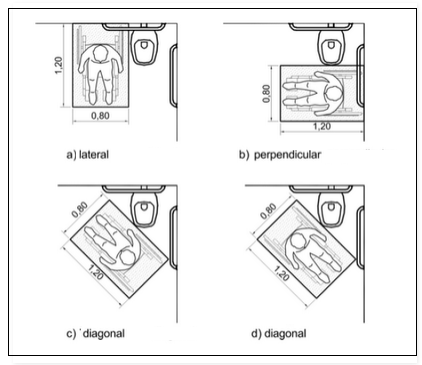
\includegraphics[width=7cm]{brazil_images/image014.png}
\caption{Regulation for accessible lavatory design}
\label{fig:regulation_accessible_lavatory}
\end{figure}


It is possible to understand from this regulation the current transfer process and the space required by the users to have their independence.\\

\noindent\emph{Lavatory of the Boing 787 Dreamliner}\\ “The Dreamliner features two wheelchair-accessible lavatories, each with significant advancements. The 56-inch longitudinal lavatory repositions the entryway door and toilet to provide extra usable space and makes it easier for passengers to reach and use the facilities. A 56-inch by 57-inch convertible lavatory includes a movable center wall that allows two separate lavatories to become one large, wheelchair-accessible facility. Other wheelchair-accessible lavatory improvements include an additional toilet-flush button on the sink cabinet and a fold-down assist bar to aid independent transfers.” \cite{2014pn}\\ 

\noindent\emph{Dual pivot expandable lavatory}\\ The lavatory may be positioned close to the doorway area of the airplane, and is provided with a primary and a secondary pivotable module. Each module is pivotally attached to a stationary assembly conventionally affixed to the ceiling and floor of the airplane. During take-off and landing both modules are locked, by means of a locking system, in a stowed position within the stationary assembly. During routine flight, the locking system is unlocked and both modules are pivoted into a deployed position within the doorway area. A flight attendant's seat may be affixed to the exterior of the primary module. If the seat is used, an additional support foot is affixed to the primary module to accommodate the additional loading on the lavatory.\cite{arnold2000dual} \\

\begin{figure}[h]
\centering
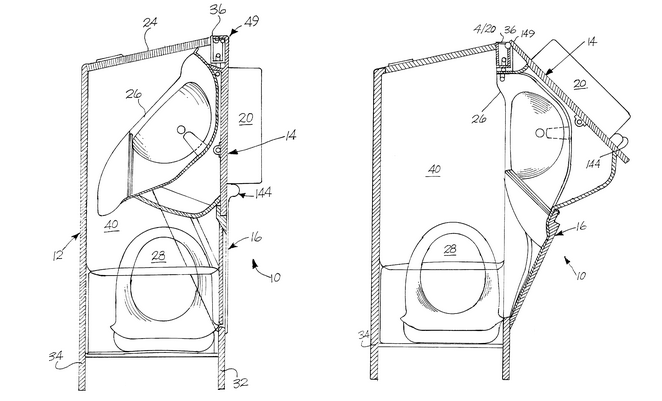
\includegraphics[width=7cm]{brazil_images/image016.png}
\caption{Dual pivot expandable lavatory}
\label{fig:expandable_lavatory}
\end{figure}

\noindent\emph{Aircraft lavatory for a person with reduced mobility}\\
 An aircraft lavatory includes first and third walls extending inwardly from a second wall and a fourth wall connecting the first wall to the third wall. A countertop extends along a portion of the first wall. A sink is disposed in the countertop. The countertop defines an under-countertop recess free from obstructions. A toilet is disposed adjacent to both the second wall and the third wall and defines a toilet axis bisecting the toilet. A door extends along at least a portion of the third wall. An access axis is defined that is disposed at an access angle with respect to the toilet axis. When a person in a wheelchair enters the lavatory area along the access axis, the countertop recess accommodates at least a portion of the person's body.\cite{grant2012aircraft}\\ 

\begin{figure}[h]
\centering
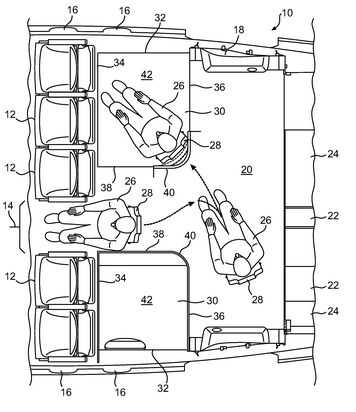
\includegraphics[width=7cm]{brazil_images/image017.png}
\caption{Aircraft lavatory for a person with reduced mobility}
\label{fig:aircraft_lavatory}
\end{figure}

We also looked for a couple of support mechanisms for the user´s foot. We decided to take this direction considering user’s feedback from the previous prototype. \\

\noindent\emph{Wheelchair support}\\
 The wheelchair support was considered as a part of the benchmarking research once it is already used for our target group. 

\begin{figure}[h]
\centering
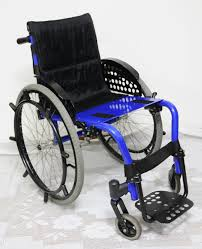
\includegraphics[width=7cm]{brazil_images/image022.jpg}
\caption{Utilitary wheelchair foot support} % - http://maonarodablog.com.br/2010/06/07/tokleve-milenium-sport-avaliacao/}
\label{fig:utilitary_wheelchair}
\end{figure}


\subsubsection{Building our prototype}

\textbf{Version 1.0} \\

The first prototype of our dark horse idea was a paper one to provide the correct vision of our product and give insights for the real scale one. In order to do that we use simple materials as paper, matchstick, clay and glue as show on \ref{fig:dark_horse_brazil}.\\

\begin{figure}[h]
\centering
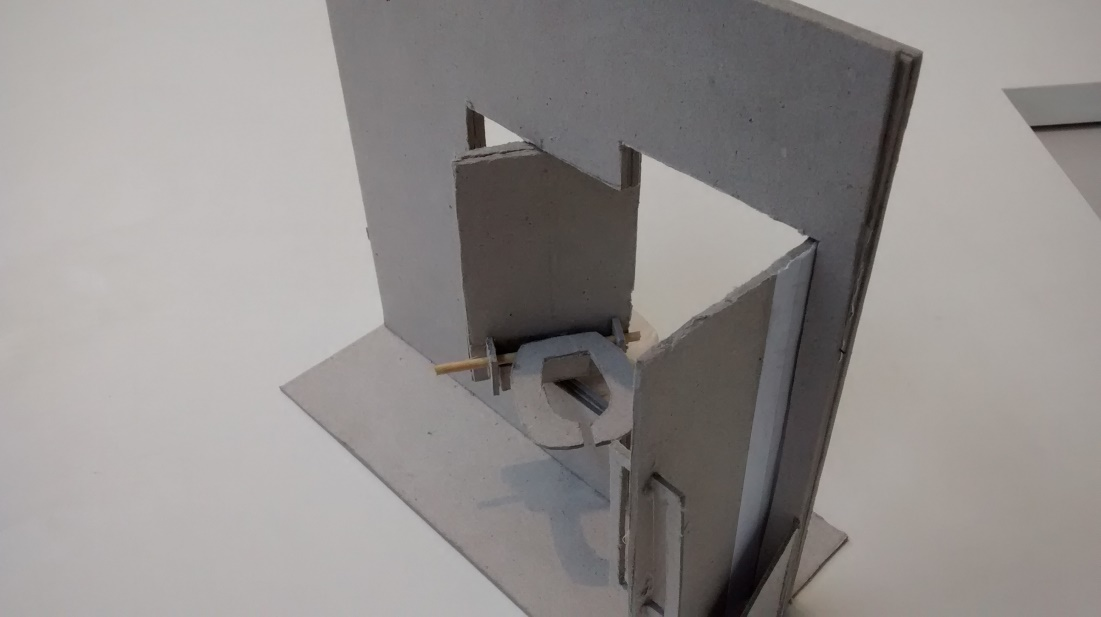
\includegraphics[width=7cm]{brazil_images/image028.jpg}
\caption{Dark horse version 1.0}
\label{fig:dark_horse_brazil}
\end{figure}

\newpage

\textbf{Version 2.0} \\

On this version of the Dark Horse we managed to make a real scale prototype to try to understand how users would react with this product and at the same time identify possible design failures and how we could improve it.

Our quest started by searching for materials that could bear the weight of a human being and also that could allow the turning mechanism to exist. A 30mm fiberboard proved to be strong enough for our needs, while the pivotable hinge provided us with the rotational movement we needed. Other than that, we used a retractable hinge to simulate the flight crews’ retractable seat.

After that we cut the fiberboard, built the prototype and tested it with some people from outside the design group, but that did not have mobility issues because our prototype was huge and heavy, it couldn’t be easy transported and because our campus has not many wheelchair users, we were not able to test it with our actual target users.\\

\begin{figure}[h]
\centering
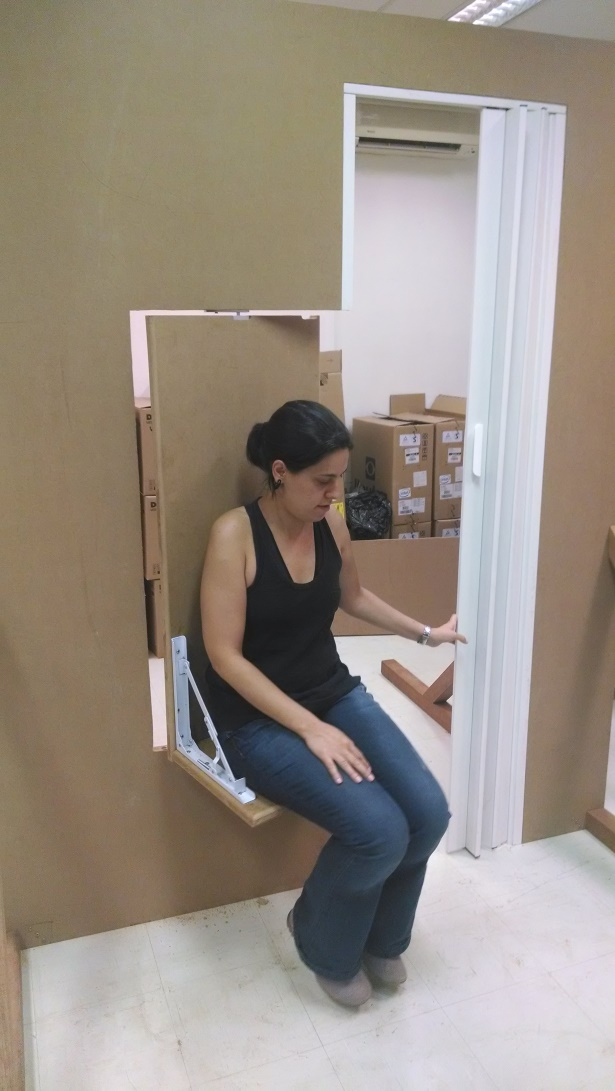
\includegraphics[width=7cm]{brazil_images/image031.jpg}
\caption{Testing with people from outside the group}
\label{fig:test_outside_group}
\end{figure}

\newpage

\textbf{Version 3.0} \\

On this version we tried to build a more complex turning mechanism that would provide greater independence for our user. Besides that we managed to create a mechanism for the feet and tested with some people outside the group with no mobility issues and asked for the opinion of one potential user. First, we printed a couple of gears and tried to create a turning mechanism and then we designed the feet mechanism and tested it with more people. \\

\begin{figure}[h]
\centering
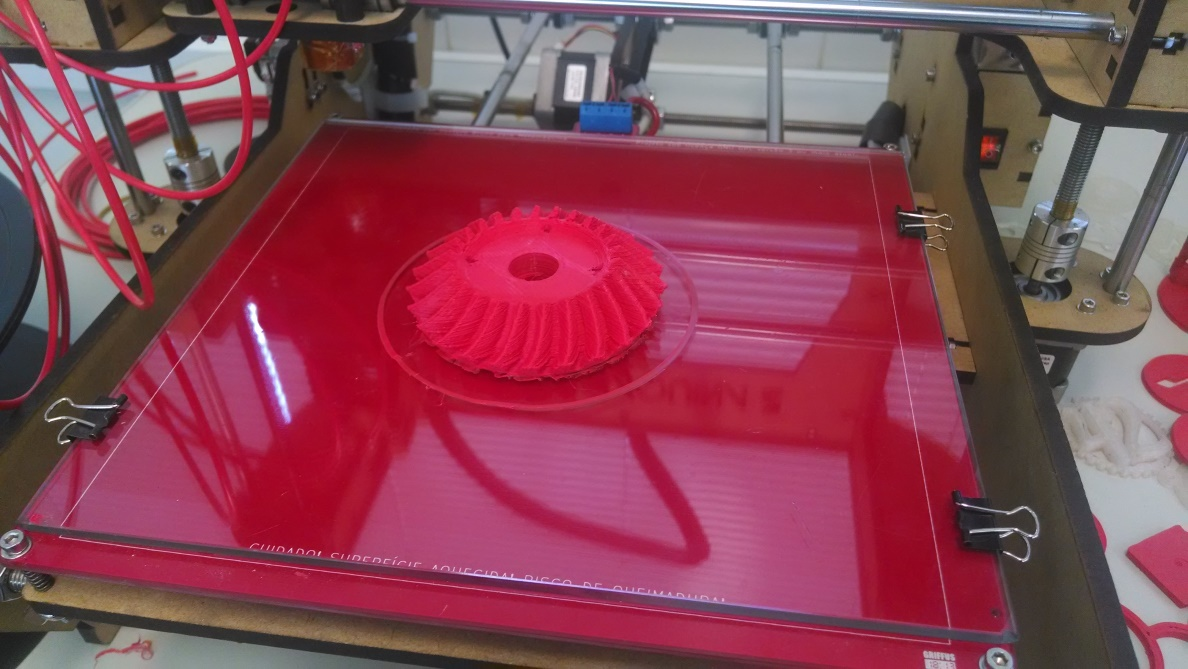
\includegraphics[width=7cm]{brazil_images/image032.jpg}
\caption{Printed gear}
\label{fig:printed_gear}
\end{figure}

\subsubsection{Learnings and Feedback}
Here are the things we learned : \\
\begin{itemize}
	\item Privacy and autonomy are of utmost importance for our users.
	\item The way that the user removes his pants needs to be thought.
	\item Rotating mechanism does not necessarily have to be motorized. It could be just a mechanic system, avoiding thus the increase in energy consumption and weight;
	\item The gap between the rotating wall and the structure wall must be sealed;
	\item Having the right tools can make the prototyping process much faster;
	\item The footrest has to allow a smooth transfer. Rotating wheels do not comply with this requirement. 
	\item Because of the friction of the wheels, the force needed to rotate the chair increases considerably. A better solution would include a “floating” adjustable footrest.
	\item 	The footrest angle must be adjusted so as to provide comfort for the user.
	\item 	The current airplane lavatories do not have enough space to accommodate the rotating toilet seat.
	\item Hygiene must be taken into consideration as you are exposing the airplane to potential pathogenic agents when the wall is rotated.
\end{itemize}

Here is the feedback we got from our users : \\

\begin{itemize}
	\item Our interviewee Cid Torquatto told us that he would actually use the solution and that it is a great way to encourage reduced mobility people use the bathroom on airplanes
	\item The seat must have more depth and be wider, because the way it is now it feels like one could fall from it
	\item Rotation mechanism is safer using a manual solution rather than an automatic one
\end{itemize}

\section{Funky Prototype}

The conclusion of Dark Horse brought the team to the beginning of the Funk-tional prototyping mission.  This mission called for the creation of a functional system that could be integrated using funky materials such as duct tape, foam core, etc. The system needed have enough functionality such that it could would answer critical questions by being tested in real time.

While our team was brainstorming about the first version of the funktional prototype, the first issue that we immediately had to deal with was defining the boundaries of our system. We wanted to make our user feel more in control of his/her environment but at the same time we realized that the word environment had a very extensive meaning that we needed to define more accurately. In order to do so, we defined our system at first as everything that happens between the departure airport gate (see Appendix B).

We thus identified three main issues :

\begin{easylist}[itemize]

& Boarding/Deboarding the plane, which we tried to address with our dark horse prototype.

& Moving through the cabin space is a huge issue, especially if passengers with reduced mobility want to use the lavatories.

& Feeling comfortable in your seat. This the big issue we decided to address for the funktional prototype. We decided to focus on the armrest because we saw it as a way to make people feel more comfortable in their seats as well as make it easy for them to access their seat but also as a place to centralize the controls (fan, light, flight attendant call, etc.) 

\end{easylist}


\subsection{Benchmarking}

The Dark Horse mission focused on the reconfiguration of the cabin to meet the passengers' needs.  For Funky, we decided to focus on how the user controls their immediate environment in the airplane and how that can be defined.  We decided to create a subsystem of the airplane chair that consisted of the seat, the TV screen in front of the passenger, the overhead bin above the head of the passenger, and the armrest on both sides.

\subsubsection{Version 1: Controlling the Environment} 
Version 1 focused on controlling the environment by changing the methods in which the passenger can use the controls or buttons at their seats.  Today, the passenger has to reach above his head on the overhead bin compartment to call the flight attendant, to change the air flow and direction, or to turn on or off the light.  This is not an ideal arrangement for our users since some of them do not have the upper body strength that is needed to lift themselves up to touch the buttons.  We decided that we needed to bring the controls down to them and make them easier to reach and more accessible.  The controls should be an assistive technology, not another aspect of the flying experience that makes our users dependent on other passengers.   

We first envisioned the controls being placed upon the armrest through buttons, scroll bars, track pads, and other mechanisms. We looked into what is being done within the business classes on most flights.  Since we are focused on the economy class, we thought that if a solution is aready present in the business class, we could just integrate that same solution into the economy class. \ref{fig:ArmrestsControls1.jpg} and \ref{fig:ArmrestsControls2.jpg} show examples of controls on the armrests.  The first set of controls is used to control the position and the firmness/softness of the seat.  We thought about integrating  something similar and giving our user the ability to change these aspects of their seat given that different disabilities have different support needs. However, we focused on having the basic controls of the lights, the air conditioning, the flight attendant button for our design. 

\begin{figure}[h]
  \centering
     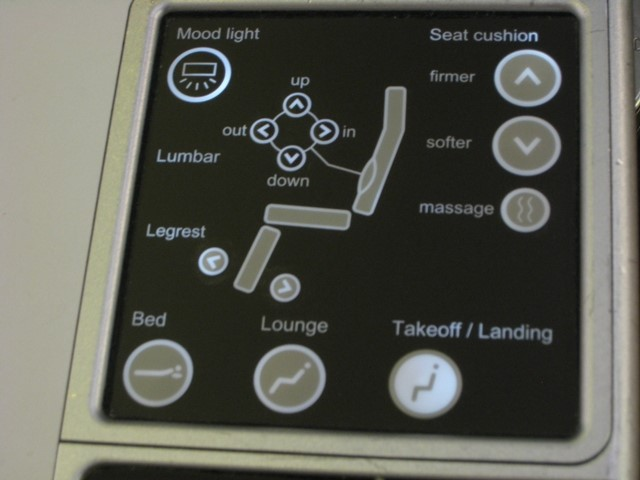
\includegraphics[width=7cm]{images/ArmrestControls1.jpg}
   \caption{Example of current controls on the armrest in a Business Class seat. \cite{armrest_controls1}}
  \label{fig:ArmrestsControls1.jpg}
\end{figure}

\begin{figure}[h]
  \centering
     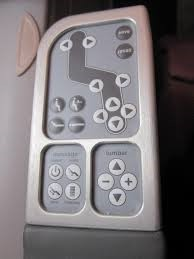
\includegraphics[width=7cm]{images/ArmrestControls2.jpg}
   \caption{Example of current controls on the armrest in a Business Class seat. \cite{armrest_controls2}}
  \label{fig:ArmrestsControls2.jpg}
\end{figure}

\ref{fig:HingedArmrest.jpg} shows a hinged armrest in which a remote control lies within the armrest compartment.  We thought about incorporating a hinged cover onto the armrest with controls, not a remote, underneath in order to protect the controls from being hit on accident during flight. We worried, however, that this would make buttons less accessible to users and they would feel that they shouldn't press them as often since they aren't in direct contact with them at all times. 

\begin{figure}[h]
  \centering
     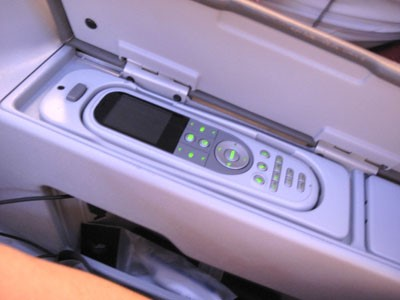
\includegraphics[width=7cm]{images/HingedArmrest.jpg}
   \caption{Hinged Armrest that could be incorporated with Control Interface. \cite{hinged}}
  \label{fig:HingedArmrest.jpg}
\end{figure}


The use of individual TV screens on airplanes is increasing due to the demand of entertainment.  We considered the use of the TV screen as another method of reaching the controls or making the controls accessible. Some TV screens have a remote associated with them while others have a touchscreen.  The primary interface we focused on was the touchscreen.  \ref{fig:TVScreenwithRemote.jpg} shows a TV screen with a remote in the economy section of an airplane.  \ref{fig:TouchscreenTV.jpg} below shows a touchscreen TV on an airplane in premium economy class. We also brainstormed one step further and considered what it would be like if the user could use their own electronic device (iPad, tablet, or phone) to manipulate the controls.

\begin{figure}[h]
  \centering
     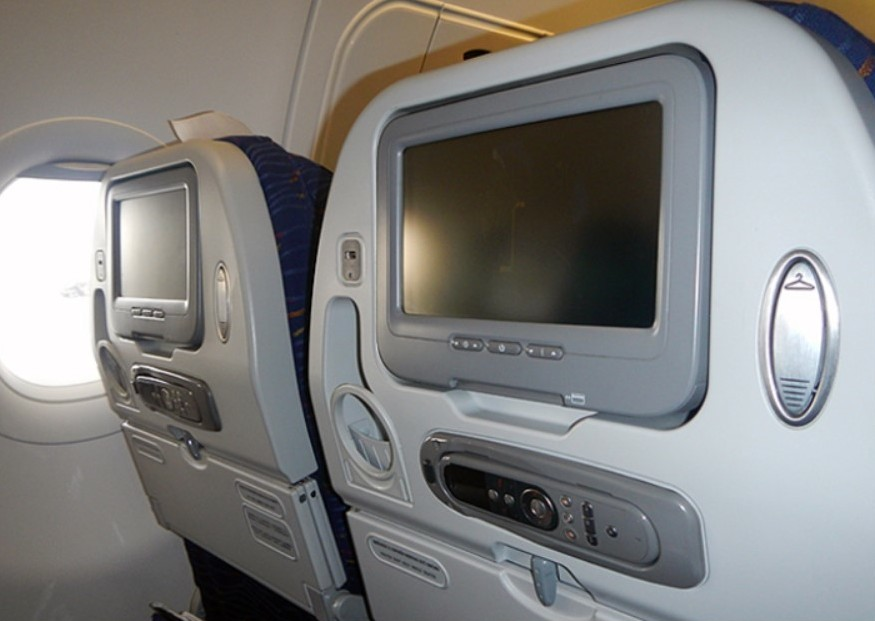
\includegraphics[width=7cm]{images/TVScreenwithRemote.jpg}
   \caption{TV screen with remote on an airplane. \cite{TVremote}}
  \label{fig:TVScreenwithRemote.jpg}
\end{figure}

\begin{figure}[h]
  \centering
     \includegraphics[width=7cm]{images/TouchscreenTV.jpg}
   \caption{Touchscreen TV on an airplane. \cite{touchscreen} }
  \label{fig:TouchscreenTV.jpg}
\end{figure}

\subsubsection{Version 2: Controlling the Environment with a New Armrest and Controls}

Version 1 on Funky showed us that there were more areas that needed to be improved within our design subsystem.  We decided that we would further develop the controls but also look into ways to redesign the armrest.  Why did the armrest have to be like it is? Can it move up and down another way? Can we design something with the same functionality but to be more accessible and more comfortable?

We looked into armrest in all sorts of transportations mediums. We needed to know what had already been done, what could be integrated together, and what we needed to design to surpass the shortcomings.   \ref{fig:SplitArmrests.jpg} below shows an armrest unit being split into two so that both persons have an armrest and it can be moved front to back by sliding on the mount to adjust to the desired arm position. This is currently being used in automobiles.


\begin{figure}[h]
  \centering
     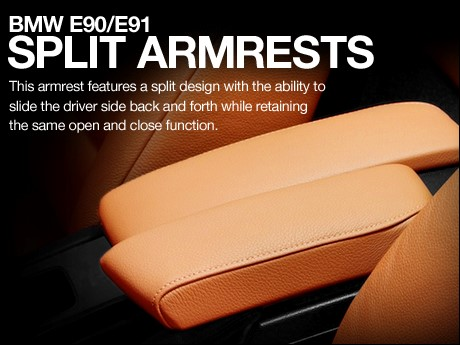
\includegraphics[width=7cm]{images/SplitArmrests.jpg}
   \caption{Split Armrests that can move relative to each other.\cite{splitarmrest} }
  \label{fig:SplitArmrests.jpg}
\end{figure}

We wanted to design the armrest so that it would not be in the way during transfer from the wheelchair into the airplane chair.  One method of doing this is shown below in  \ref{fig:LoungerArmrest.jpg}.  The armrest are part of the lounger and then pop out when the lounger changes positions.  We wanted to integrate a similar concept into the airplane chair but knew that we would have to consider a way that was slightly more complex than the mechanism below due to the fact that economy seats do not lay down or recline enough for this mechanism to be feasibly implemented. 


\begin{figure}[h]
  \centering
     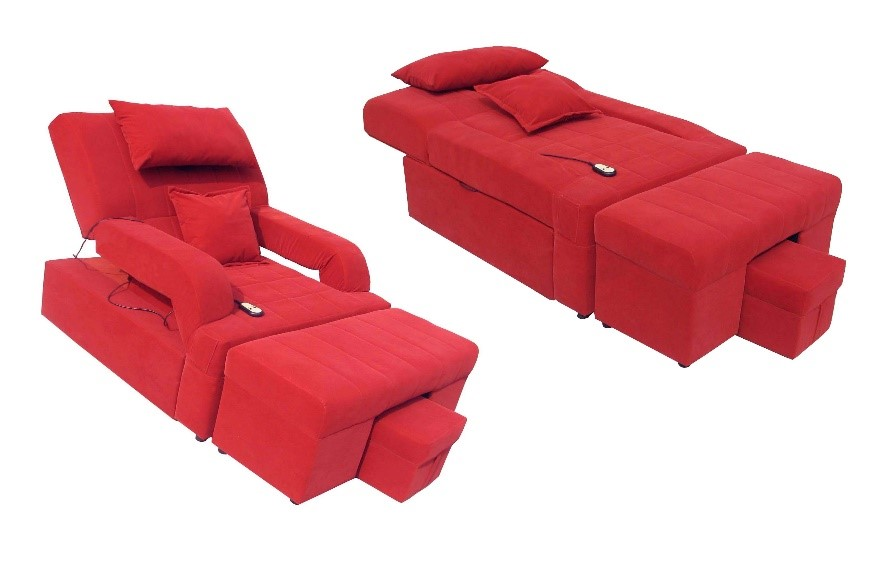
\includegraphics[width=7cm]{images/LoungerArmrest.jpg}
   \caption{Lounger with Built-In Armrests \cite{lounger}}
  \label{fig:LoungerArmrest.jpg}
\end{figure}


Another method of moving the armrest out of the path of transfer would be to have them hydraulically move in the horizontal or vertical plane. \ref{fig:dentalchairarmrest.jpg} below shows armrests on a dental chair that can be hydraulically moved for personal preference and to allow easier transfer to the seat. Similar technology to the hydraulic movement is the lifting and lowering of an office chair using air pressure and a piston.   



\begin{figure}[h]
  \centering
     \includegraphics[width=7cm]{images/dentalchairarmrest.jpg}
   \caption{Dental Chair With Hydraulic Armrests to Position where desired. \cite{dental}}
  \label{fig:dentalchairarmrest.jpg}
\end{figure}

For a more futuristic armrest, we looked into design concepts and luxury seating.  \ref{fig:FrontArmrests.jpg} below shows a design concept for an airplane chair and business space.  The chair has armrests that come from the front and could be lifted and lowered from under the seat.  These armrests allow for a wide range of lifting and lowering mechanisms as well as more flexibility with controls that could allow the weight of the controls to be beneath the cabin.


\begin{figure}[h]
  \centering
     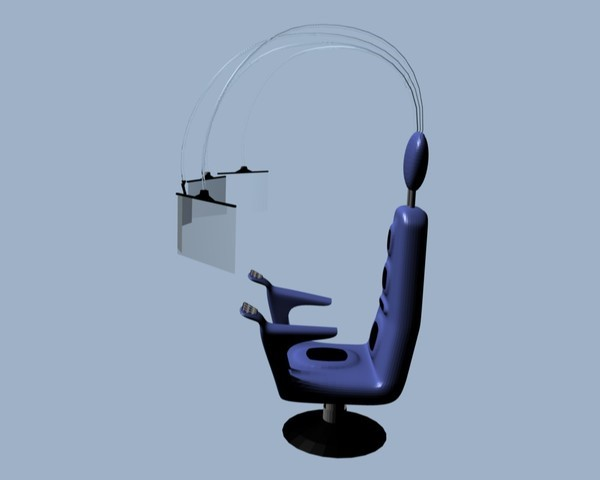
\includegraphics[width=7cm]{images/FrontArmrest.jpg}
   \caption{Armrests Located on the Front of the Seat. \cite{frontarmrests}}
  \label{fig:FrontArmrests.jpg}
\end{figure}

Massage chairs were the luxurious chairs that we considered.  \ref{fig:MassagerArmrests.jpg}  below displays an armrest that has the controls on the top and a spot for your arm inside a protective C-shaped area. This design allows for the comfort of knowing which armrest is yours and not bumping or touching the other person beside you.  It also has the controls easily accessible without the fear of accidentally hitting them and signaling for the flight attendant or cranking the volume up to an uncomfortable setting.

\begin{figure}[h]
  \centering
     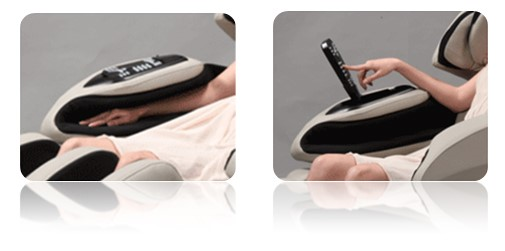
\includegraphics[width=7cm]{images/MassagerArmrest.jpg}
   \caption{ The luxurious armrest of a massager with controls and a designated arm place. \cite{massage}}
  \label{fig:MassagerArmrests.jpg}
\end{figure}
 
 
The final area we researched was the armrest aids for persons with limited mobility or senior adults.  One such device is shown below in \ref{fig:AssistiveArmrests.jpg}.  This device allows for the user to be aided in seating on the toilet and raising from the toilet.  This device would be applicable for both the chair armrest situation as well as the airplane bathroom accessibility situation. The mechanism for this device follows an arc trajectory during use. This arc trajectory aids passengers that have limited mobility and difficulty seating and standing by allowing them to have a device that moves in a path similar to their mass center. This armrest would be useful for limited mobility passengers that could walk short distances and are not confined to a wheelchair.

\begin{figure}[h]
  \centering
     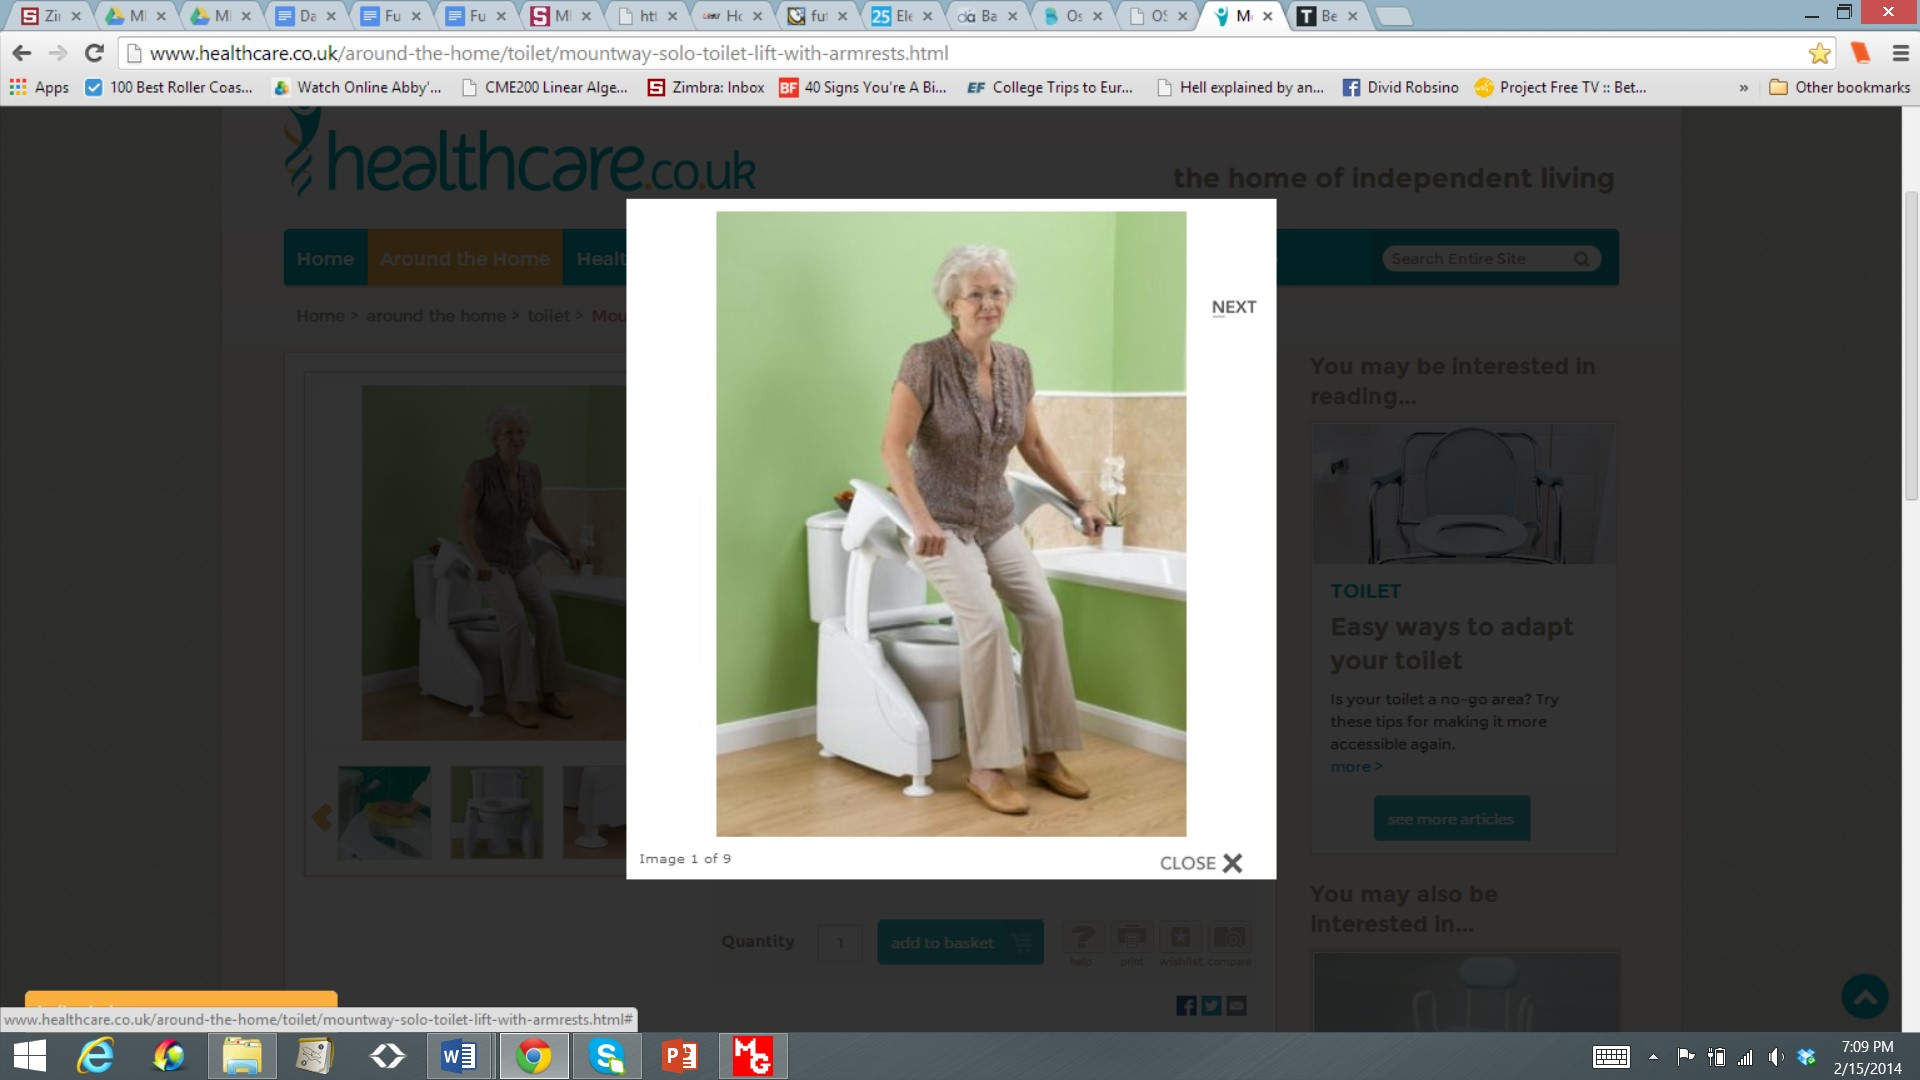
\includegraphics[width=4cm]{images/AssistiveArmrest.jpg}
   \caption{ Lifting and Lowering Armrest Mechanism for the Elderly. \cite{toilet}}
  \label{fig:AssistiveArmrests.jpg}
\end{figure}


\subsection{Description of the prototype}


\subsubsection{Controls}

Funky allowed us to create different interfaces for interacting with the cabin controls in order to examine the level of independence and control a person with reduced mobility experiences with each. After speaking to our users, we know that reaching the controls on the ceiling can be very hard, especially if a passenger does not have much upper body strength. Thus, we wanted to find a way to bring the controls to them and minimizing the effort exerted into changing their cabin environment.  Our team focused on 4 main areas for inputs shown in Figure \ref{fig:ControlArchitecture.jpg}: buttons on the armrest, GUI on screen, GUI on personal device and automated controls.  On the backend, we had an Arduino controlling the lights, the fan and the flight attendant light. 


\begin{figure}[h]
  \centering
     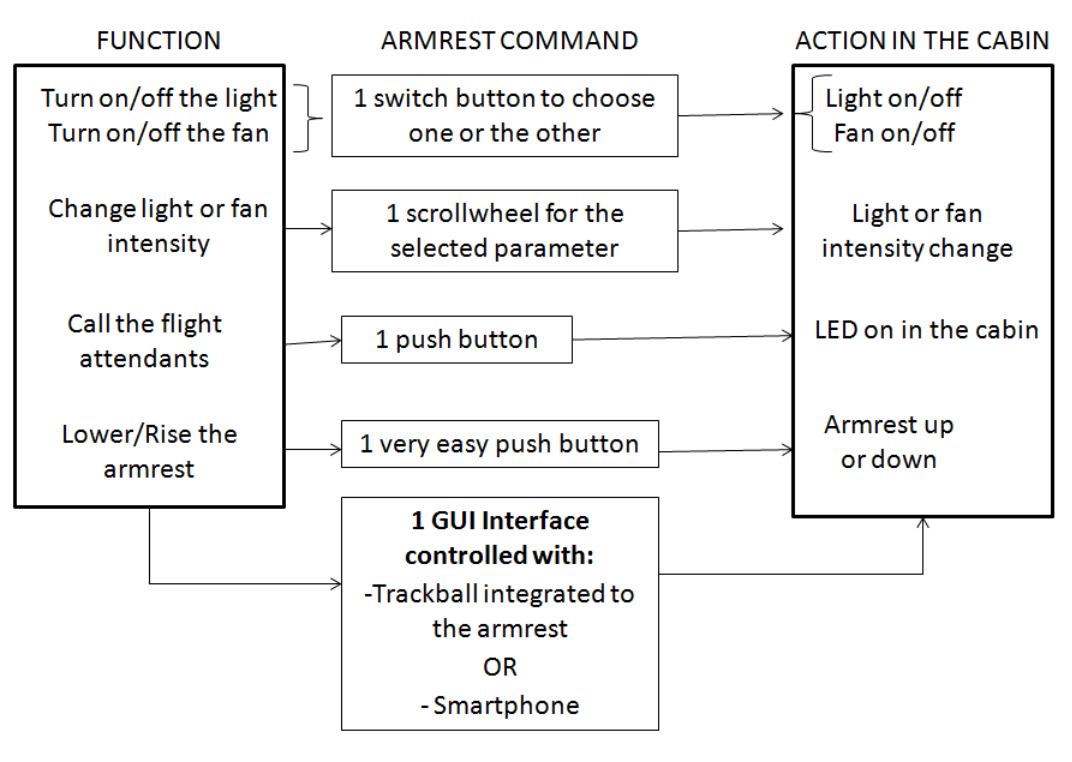
\includegraphics[width=10cm]{images/ControlArchitecture.jpg}
   \caption{Architecture of the system we wanted to build to offer a centralized and better control of the environment to our user}
  \label{fig:ControlArchitecture.jpg}
\end{figure}

\subsubsection{Buttons on armrest}

\begin{figure}[h]
  \centering
     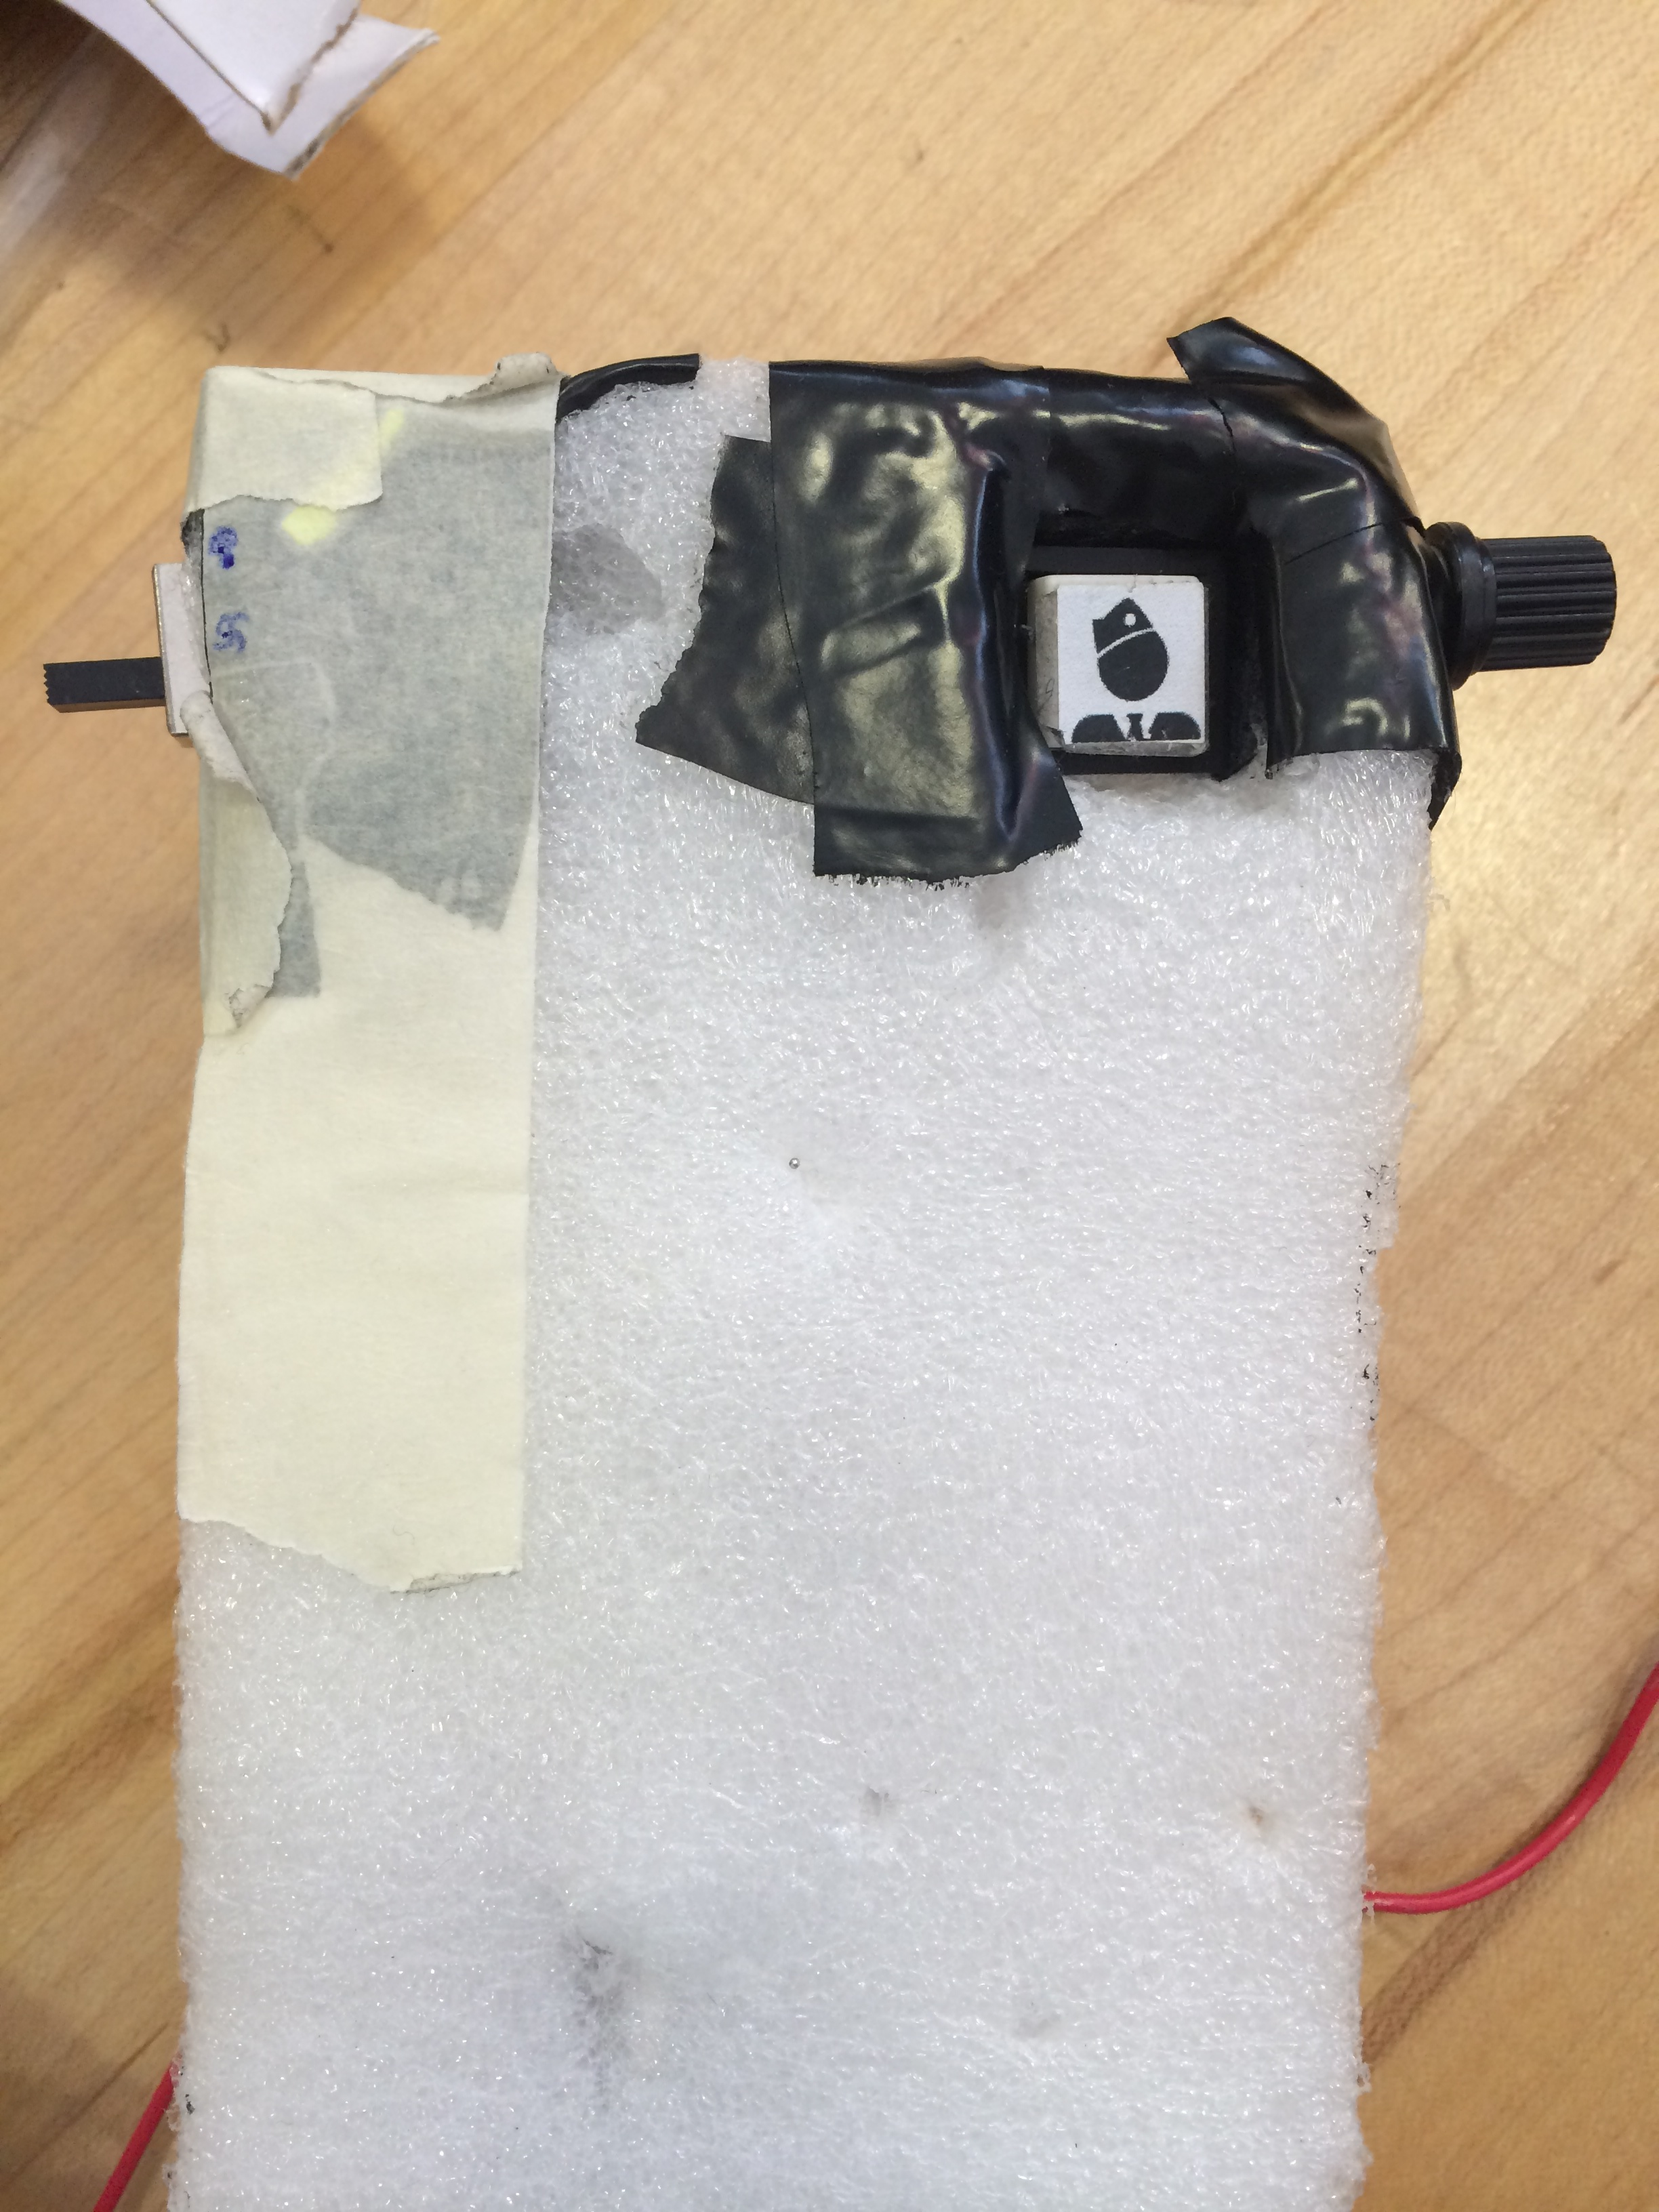
\includegraphics[width=4cm]{images/FoamArmrest.jpg}
   \caption{ Prototyped armrest with integrated buttons}
  \label{fig:FoamArmrest.jpg}
\end{figure}

Since passengers are already accustomed to using buttons to change their environment or summon the flight attendant, we decided to bring these buttons closer to them and test the type of input that was more intuitive to the desired output. The final iteration is shown in  Figure \ref{fig:FoamArmrest.jpg}. The location of these inputs is key- we want them to be readily accessible when the user needs them but “invisible” enough such that the user does not accidentally press them. 

After testing different locations for each button, we decided that all of them should be placed on the side of the armrest (so they are not accidentally triggered) with markings on the top of the armrest so it is easy to determine the function of each. However, the flight attendant button was actually to remain on the top of the armrest except inserted into an inlet so that once would intentionally have to go into a lower plane to press the button. We tested buttons for both the fan and the lights but realized that it was more intuitive to use a potentiometer to control both of these functions, especially so the user could control the intensity of both. A switch would toggle between fan and light functionality, much like how you choose your right or left rear view mirror to be adjusted in your car.  

While the set up for all the inputs was designed on the armrest, there were unfortunately technical complications we did not foresee and were thus unable to fully test out this prototype. \\

\subsubsection{GUI on Screen and Device}
In order to test whether users were more comfortable with a Graphic User Interface (GUI) as opposed to physical buttons, we created a GUI on MATLAB, loaded it on to a table and connected this to our Arduino. The GUI, shown in Figure \ref{fig:MATLABGUI.jpg}, has the ability to control the lights, the fan, and the flight attendant call button.

\begin{figure}[h]
  \centering
     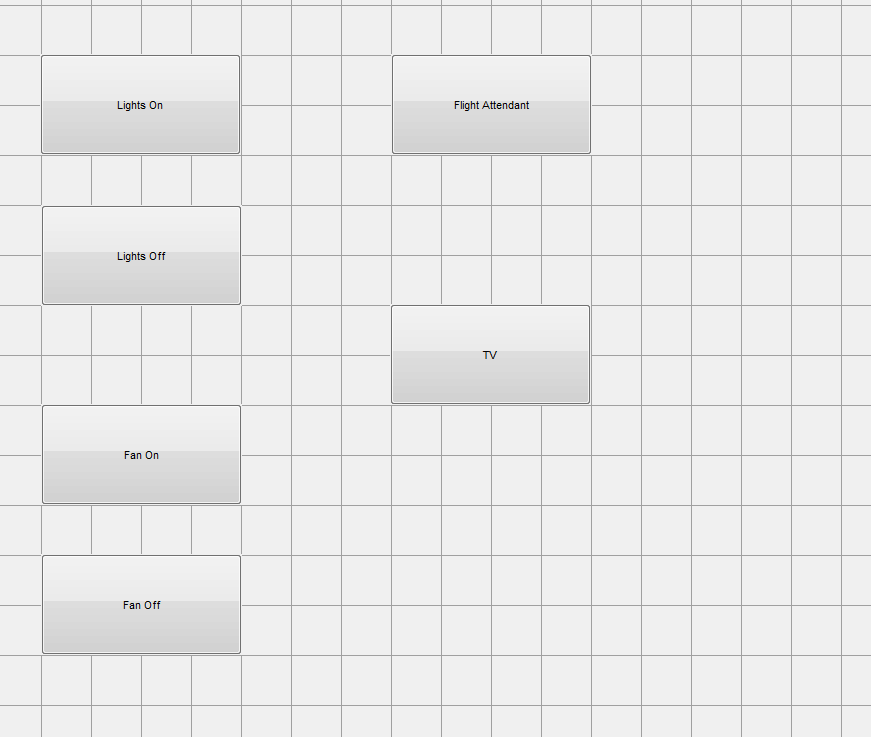
\includegraphics[width=12cm]{images/MATLABGUI.jpg}
   \caption{ GUI that controls the lights, fan and flight attendant call button. }
  \label{fig:MATLABGUI.jpg}
\end{figure}

This GUI was utilized two test two different scenarios, having the ability to control the GUI as if it was placed on the seatback of the seat in front of you with both touch and with the trackball shown in Figure \ref{fig:Trackball.jpg} as well as having the user controlling it with their hands as if they were using your own device. 

\begin{figure}[h]
  \centering
     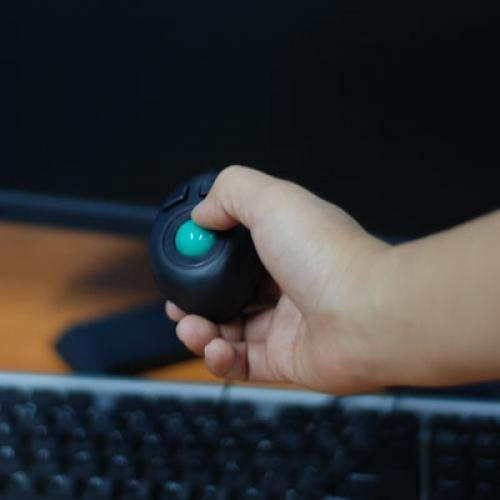
\includegraphics[width=7cm]{images/Trackball.jpg}
   \caption{ Trackball used to control GUI on seatback of seat in front of you. }
  \label{fig:Trackball.jpg}
\end{figure}


\subsubsection{Automated Controls}

After exploring different inputs a user could trigger to control their environment, our team decided to take a step back and go back to the basics. Why does a user want to turn their light on? Why do they want their fan off? It seemed to us that there are specific needs a user is trying to satisfy when changing these aspects of their environment, so what if the cabin could anticipate these needs and change the cabin for them? Would they still feel in control and independent? 

We decided to test out our hypothesis by assuming that people want to turn on the lights when they want to read. Therefore, if a passenger brings out a book, the light should automatically turn on. We tested this by using an image detection algorithm in MATLAB that would use the camera to detect if a certain color was present and would then trigger a command to turn the light on. We then got a light blue book and used this program to turn the lights on when the book appeared and off when the book disappeared. While this is not incredibly reliable or robust at the moment, we envisioned that if the cabin could sense when you had paper, or text or even your hands in a certain “reading” position, the light would turn on. Similarly, we could imagine using different types of remote or tactile temperature sensors to control the fan.

\subsubsection{Armrest}
After our research into different types of armrests we decided to prototype one we hadn't seen - an armrest that can collapse downwards into the space between two seats. There were several reasons for pursuing this design, including that the controls would still be reachable and that the user could raise and lower the armrest without having to twist their body.

Our prototype, shown in Figure \ref{fig:armrest_funky}, was constructed primarily from an Ikea Alrik swivel chair, which provided the mechanism for linear actuation. We sawed off the sides of the seat, using what remained as the physical armrest. Because the chair is designed for a person to sit on we also added springs to make it easier to lower the armrest without applying as much force.


\begin{figure}[h]
  \centering
     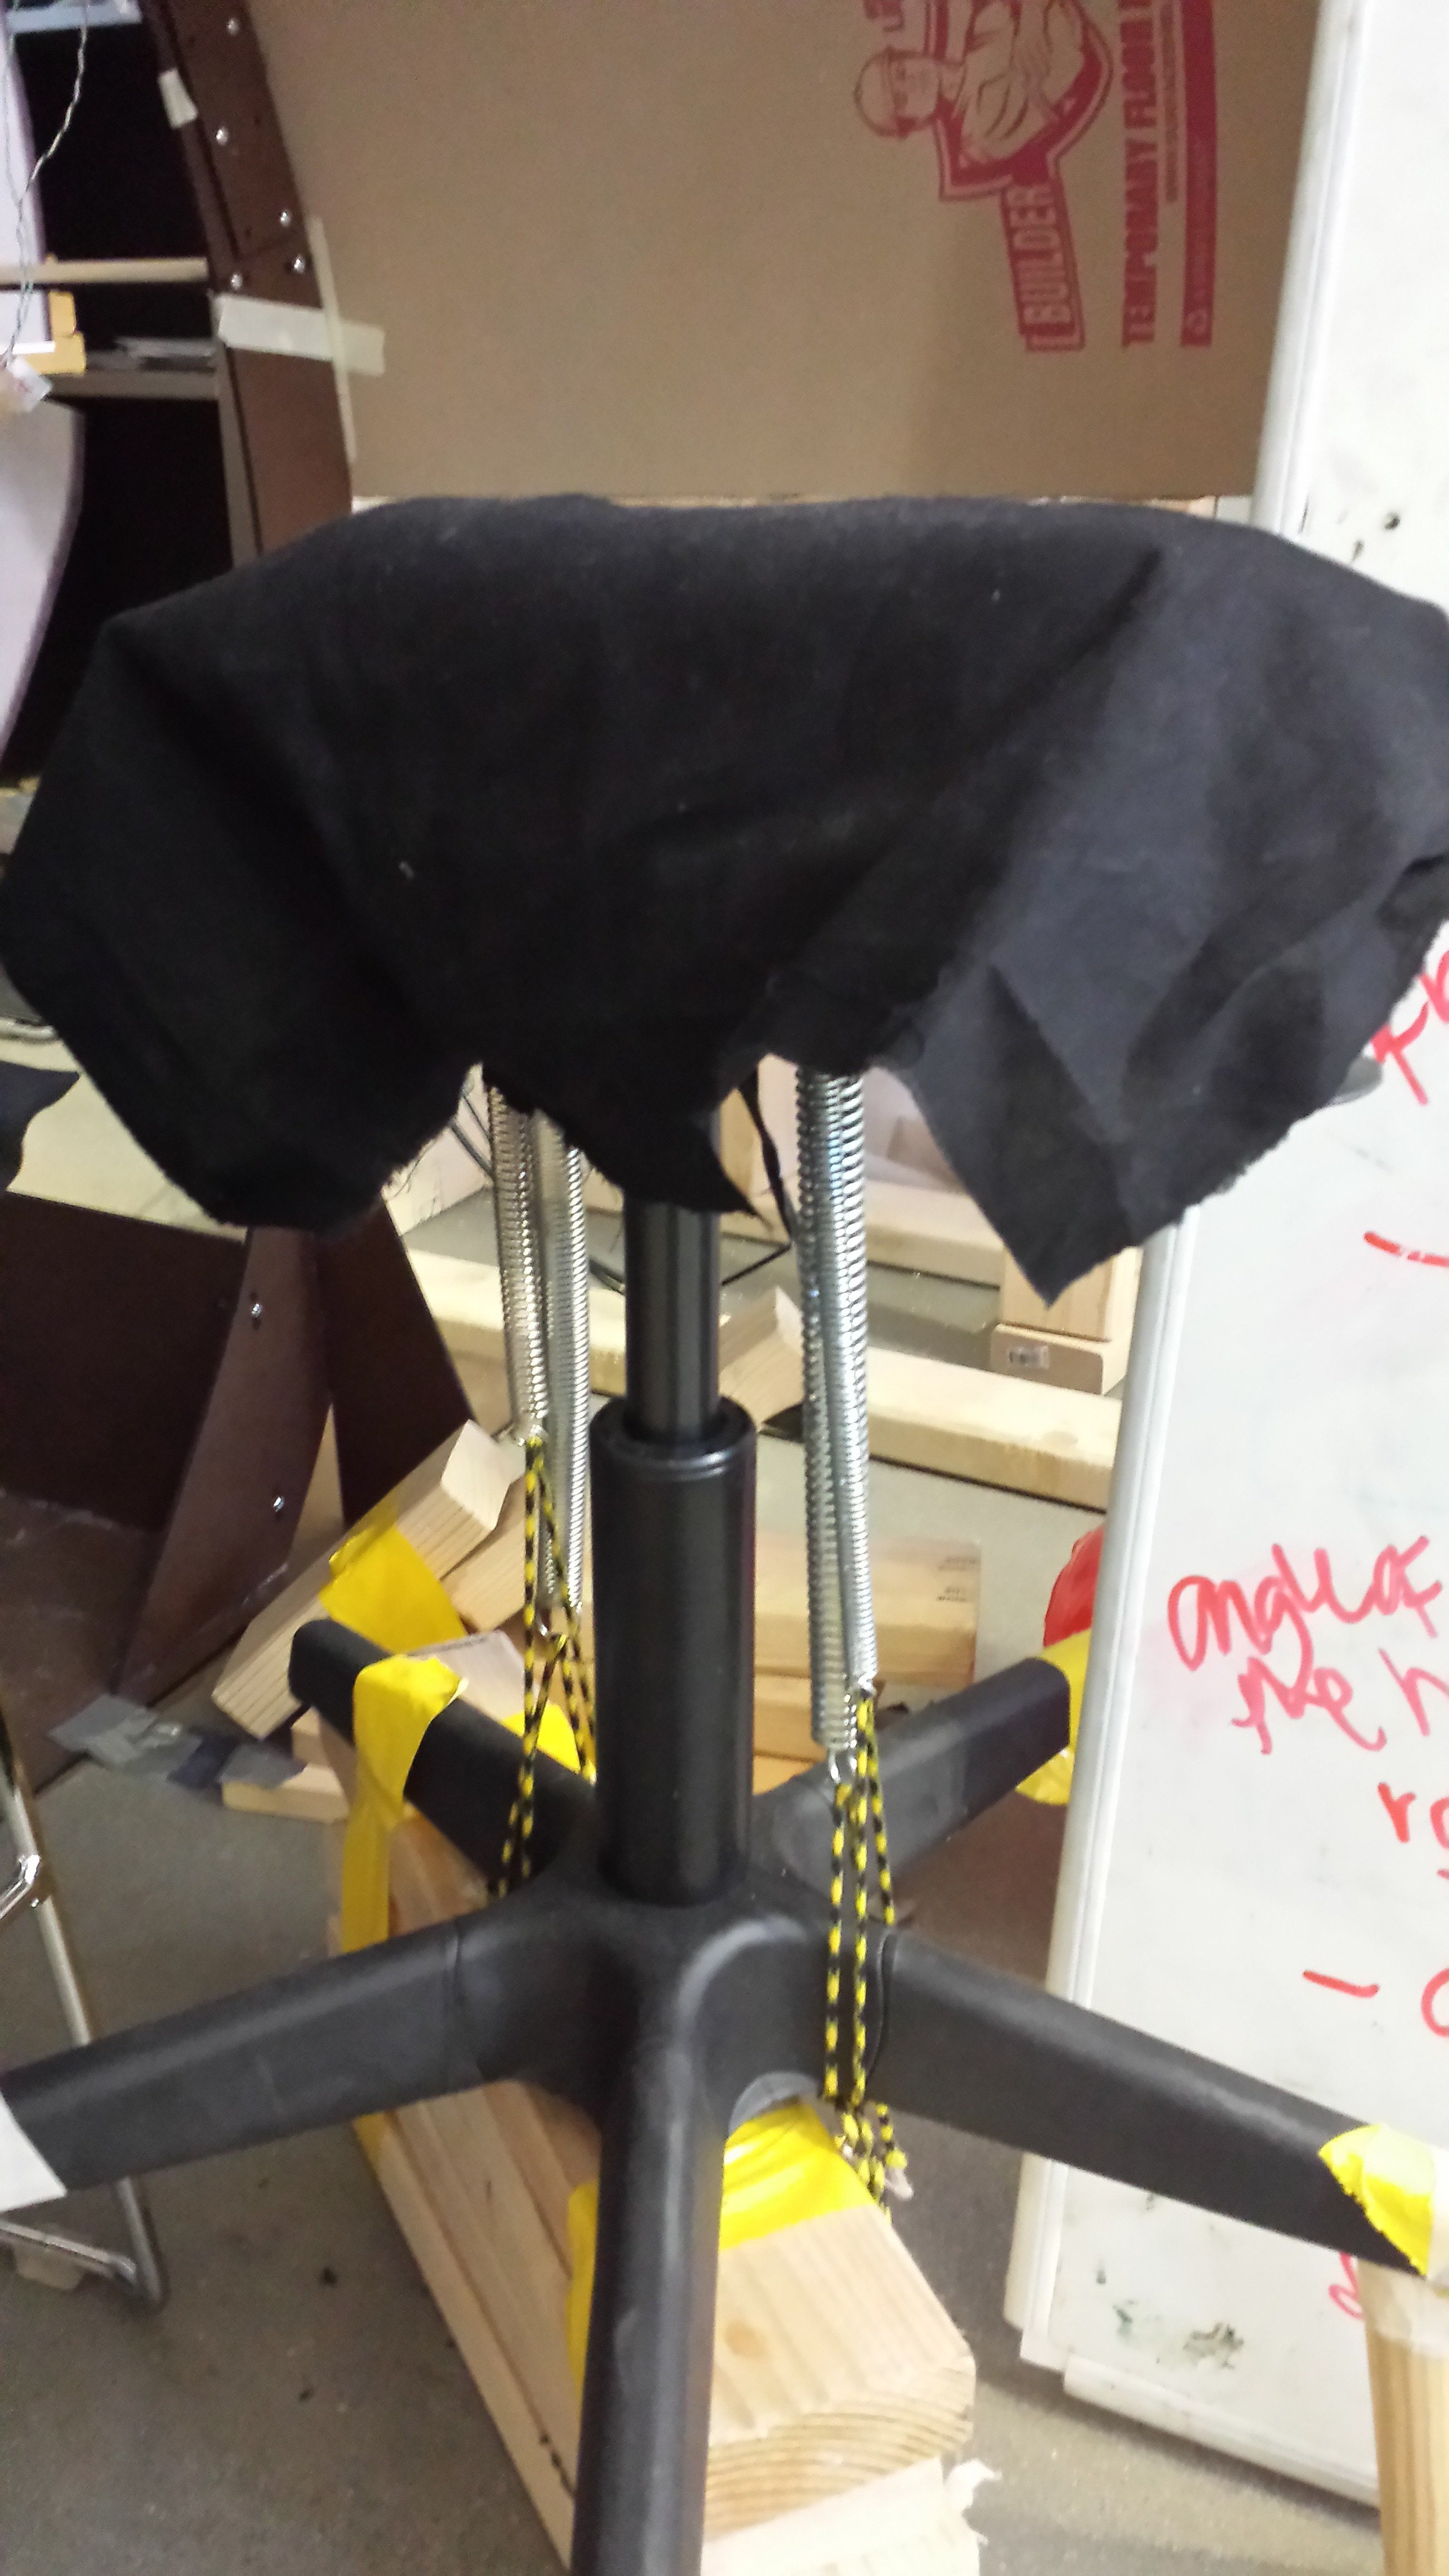
\includegraphics[width=7cm]{images/armrest_funky.jpg}
   \caption{Funky armrest prototype}
  \label{fig:armrest_funky}
\end{figure}


\subsection{Learnings}

Funky version 1 taught us that it is very important to define our goals and our vision before trying to build anything. We took time to precisely define what problems we wanted to tackle and it allowed us to get a very nice result for the second version of our prototype.

Version 2 of the funky prototype was the direct evolution of version 1 since we decided to keep focusing on the controls and to bring this idea and concept as far as we could. Since we had designed different devices to control the user's environment (buttons on the armrest, trackball, smartphone/tablet app,...) we wanted to know which one was the best for a disabled passenger and we asked one of them to come and test our prototypes.

We invited José Luis Naranjo Montoya, a 28 year old T6-complete paraplegic to share our vision with him and to get user's feedback about our version 2 funky prototype which was made of two parts : the armrest and the mechanism we designed to make it lower and raise, and the controls of the environment that we wanted initially to centralize in the armrest.

\subsubsection{User's feedback about the armrest mechanism we designed:}

When we decided to redesign the armrest and the mechanism that makes it lower and raise, we identified two main functions for the armrest: rest the passenger's arm and divide the space. But while testing our mechanism with José we realized that we had neglected one very important function of the armrest : being used as a handle by people with reduced mobility. Indeed, disabled people often use the armrest as a handle for support when they get in the cabin and shift in their seat. Therefore the armrest has to be reliable since our user relies on it to support his/her weight, and this is obviously something we learnt from José and that made us change our design priorities concerning the armrest.

Another important point we also learned from José was about the location of the armrest. It needs to be flush with the seats when it is lowered otherwise it doesn't make getting into the seats that much easier. This can seem to be in contradiction with the previous point since on the one hand our user uses the armrest as a handle but on the other hand he does not want it to be an obstacle between him and his seat. In fact, ideally our user would like to have the aisle armrest flush with the seat but the other armrest up to use it as a handle. For our user the two armrest are not equal and this way of thinking opened for us a whole new design space. 


\subsubsection{User's feedback about the control systems we designed:}

\begin{easylist}[itemize]

& Buttons in the armrest: Potentially problematic as limited mobility users prefer to have something to hold on to that is sturdy when they move themselves. However, buttons are a good way to access quickly a function (light or fan) and could be used as a redundant system or a complement of a fully automated system that could happen to fail.

& Trackball to control a GUI that is on the screen in front of the passengers: the trackball itself is clumsy to use and requires a lot of precision from the user. This is not ideal for quadriplegic users who only have partial sensitivity in their fingers. For them it is more intuitive to tap on a touchscreen or a tablet.

& Touchscreen which could be a smartphone/tablet belonging either to the passenger or the airline: It seems that holding the device is not as easy as expected and our user would prefer to have it in front of them where the normal screen in the plane is. But in this case, the use of the screen requires the passenger to lean forward to touch it which may be hard for someone who does not have a lot of core strength due to his/her handicap.

& Cabin anticipating the user's need: we were not able to test our concept of a thermal camera which, by analysing the passenger's body temperature, can turn the fan on and off if the passenger is hot or cold. However, we were able to test our idea of a webcam detecting the presence of a book and sending the right information to turn the light on. José really liked this idea. He did not see it as an assistive technology that makes him lose his independence but really as an assistive technology that makes him independent from the others. He does not need to ask someone to turn the light on for him, the cabin has anticipated his need and the gesture that causes the light to turn on comes from him directly so he does not feel it as a loss of control on his environment. However, he mentioned that it would probably need redundant controls since autonomous systems have too many cases to work perfectly in and people would not trust it.

\end{easylist}
